\documentclass[12pt,a4paper]{ctexart}

\usepackage[a4paper,margin=2.2cm]{geometry}
\usepackage{graphicx}
\graphicspath{{docs/}{./}}
\usepackage{float}
\usepackage{booktabs}
\usepackage{longtable}
\usepackage{array}
\usepackage{multirow}
\usepackage{caption}
\usepackage{subcaption}
\usepackage{hyperref}
\usepackage{xcolor}
\usepackage{enumitem}
\usepackage{titlesec}
\usepackage{fancyhdr}
\usepackage{amsmath}
\usepackage{tabularx}

\hypersetup{
  colorlinks=true,
  linkcolor=black,
  urlcolor=blue,
  citecolor=black
}

\pagestyle{fancy}
\fancyhf{}
\fancyhead[L]{SXQ-RV32IM-CPU 设计报告}
\fancyhead[R]{\thepage}
\renewcommand{\headrulewidth}{0.4pt}
\setlength{\headheight}{15pt}

\titleformat{\section}{\Large\bfseries}{\thesection}{0.8em}{}
\titleformat{\subsection}{\large\bfseries}{\thesubsection}{0.8em}{}
\titleformat{\subsubsection}{\normalsize\bfseries}{\thesubsubsection}{0.8em}{}

\setlist[itemize]{leftmargin=2em}
\setlist[enumerate]{leftmargin=2em}

\begin{document}

\begin{titlepage}
    \thispagestyle{empty}
    \centering

    \vspace*{1.0cm}
    
\includegraphics[width=0.42\textwidth]{figures/logo.png}

    \vspace{1.6cm}
    {\zihao{2}\heiti 第十届\par}
    \vspace{0.5cm}
    {\zihao{2}\heiti 全国大学生集成电路创新创业大赛\par}

    \vspace{2.2cm}
    \begin{tabular}{p{3.6cm}p{9.2cm}}
        \zihao{4}\heiti 报告类型： & \zihao{4}\heiti 设计报告 \\[0.55cm]
        \zihao{4}\heiti 参赛杯赛： & \zihao{4}\heiti 七星微杯 \\[0.55cm]
        \zihao{4}\heiti 作品名称： & \zihao{4}\heiti RV32IM 低面积低功耗高性能中央处理器设计与 FPGA 实现 \\[0.55cm]
        \zihao{4}\heiti 队伍编号： & \zihao{4}\heiti CICC1003857 \\[0.55cm]
        \zihao{4}\heiti 团队名称： & \zihao{4}\heiti 时序泉队 \\
    \end{tabular}

    \vfill
\end{titlepage}

\tableofcontents
\clearpage

\section{项目重要内容预览}

\subsection{项目摘要}
本项目面向 FPGA 平台实现一颗自研的 RV32IM处理器，探索适用于真实场景中小型设备的前端、控制流处理和数据相关处理优化方法，形成一种在较低资源开销下实现更高性能的 CPU 设计方案。项目覆盖了从微架构设计、Verilog 建模、仿真验证到 FPGA 落地实现的完整流程。最终通过创新设计，成功实现了一颗工作在 100MHz 下的 RV32IM单发射准六级流水线 CPU。其上CoreMark 达到 275.9 Iter. / sec，整体性能已达到单发射处理器中的较高水平；同时，通过创新设计省去各类复杂大表结构，LUT 消耗仅为 3581 个；动态功耗仅为 0.231 W，热裕量达到 $58.5\,^\circ\mathrm{C}$，体现出较好的低功耗与热稳定性。总体上，该版本基本实现了小面积、低功耗、高性能的设计目标。

\subsection{核心创新设计}
\begin{itemize}
    \item \textbf{动态压缩前端机制}：以六级流水线（PREIF-IF-ID-EX-MEM-WB）为基础流水线架构，引入压缩前端机制，利用双口BRAM特性，实现无损极少额外资源使用的流水线级数五、六级数间的自主动态切换功能，为后续针对跳转分支预测的优化打下基础。
    \item \textbf{低资源跳转分支预测机制}：利用压缩前端机制，在不引入复杂ICache的前提下，将指令本身引入跳转分支预测。使得完成设计：

\begin{table}[H]
    \centering
    \begin{tabular}{|c|c|c|}\hline
 跳转分支指令类型& 跳转分支是否执行判断方式&跳转分支目标地址判断方式\\\hline\hline
         Jump Type(Jal)&  全部Taken& 直算(PC + IMM)\\\hline
         Jump Type(Jalr)&  全部Taken& JTB / RAS\\\hline
         Branch Type&  BHT(2BC) / BTFNT& 直算(PC + IMM)\\ \hline
    \end{tabular}
    \caption{跳转分支预测模式表}
\end{table}
    \item \textbf{针对分支跳转指令的Load-Use晚转发}：对依赖前一条 \texttt{LOAD} 的分支跳转指令做定向后移解析，使得在时序路径最优的前提下解决绝大部分Load-Use Hazard带来的Stall周期损失。
    \item \textbf{针对IMEM与DMEM的访存前移}：由于IMEM与DMEM均使用BRAM，故访存具有至少一拍延迟。本设计通过识别并将针对IMEM与DMEM的访存操作前移至EX阶段，将原本最多两拍Stall周期浪费压缩至最多一拍浪费。
    \item \textbf{针对乘法器的操作前移}：本设计采用FPGA板上DSP资源实现MUL相关指令。通过识别并前移一拍DSP乘法指令输入，在时序路径最优的前提下压缩一拍DSP乘法器分周期执行带来的延迟。
\end{itemize}
\newpage

\subsection{当前关键指标概览}
注：本设计采用CoreMark、Dhrystone、Embench(wikisort)三个BenchMark来综合评判CPU性能。以CoreMark为主要性能评估依据，Dhrystone与Embench为辅助性能评估依据。CoreMark 分数来自 \texttt{ITERATIONS=5000} 的实际上板 UART 输出；CoreMark 的周期数、退役指令数、IPC 以及跳转分支预测准确率来自 \texttt{ITERATIONS=1} 的 Vivado 仿真统计，用于在合理仿真时间内获得周期级微架构指标。
\begin{table}[H]
      \centering
      \caption{当前版本关键指标}
      \begin{tabular}{lll}
          \toprule
          类别 & 指标 & 当前结果 \\
          \midrule
          基本信息与指标 & FPGA设备型号 & \texttt{xc7a100tcsg324-1}\\
           & 主频 & \texttt{100MHz} \\
           & LUT / FF / BRAM / DSP & \texttt{3581 / 2741 / 16 / 4} \\
           & IPC(CoreMark) & \texttt{0.851}\\
           & IPC(Dhrystone) & \texttt{0.907}\\
           & IPC(Embench-wikisort) & \texttt{0.786} \\
          \midrule
          功耗统计 & 总片上功耗 & \texttt{0.329W} \\
           & 动态功耗 & \texttt{0.231W} \\
           & 静态功耗 & \texttt{0.099W} \\
           & 结温 & \texttt{26.5}$\,^\circ\mathrm{C}$ \\
           & 热裕量 & \texttt{58.5}$\,^\circ\mathrm{C}$ \\
          \midrule
          BenchMark评分 & CoreMark & \texttt{275.9 Iterations / sec} \\
           &  & \texttt{2.759 Iterations / MHz} \\
           & Dhrystone & \texttt{166000 Dhrystone/Sec}\\
 & &\texttt{0.945 DMIPS/MHz}\\
           & Embench-wikisort & \texttt{122.58} \\
          \midrule
          预测统计(CoreMark) & JAL 方向预测准确率 & \texttt{100.00\%} \\
           & JAL 目标预测准确率 & \texttt{100.00\%} \\
           & JALR 方向预测准确率 & \texttt{100.00\%}\\
           & JALR 目标预测准确率 & \texttt{99.91\%} \\
           & B 指令方向预测准确率 & \texttt{87.06\%} \\
           & B 指令目标预测准确率 & \texttt{100.00\%} \\
           & 总体预测准确率 & \texttt{88.43\%} \\
          \bottomrule
      \end{tabular}
  \end{table}

\section{CPU 架构设计说明}
\begin{figure}[H]
    \centering
    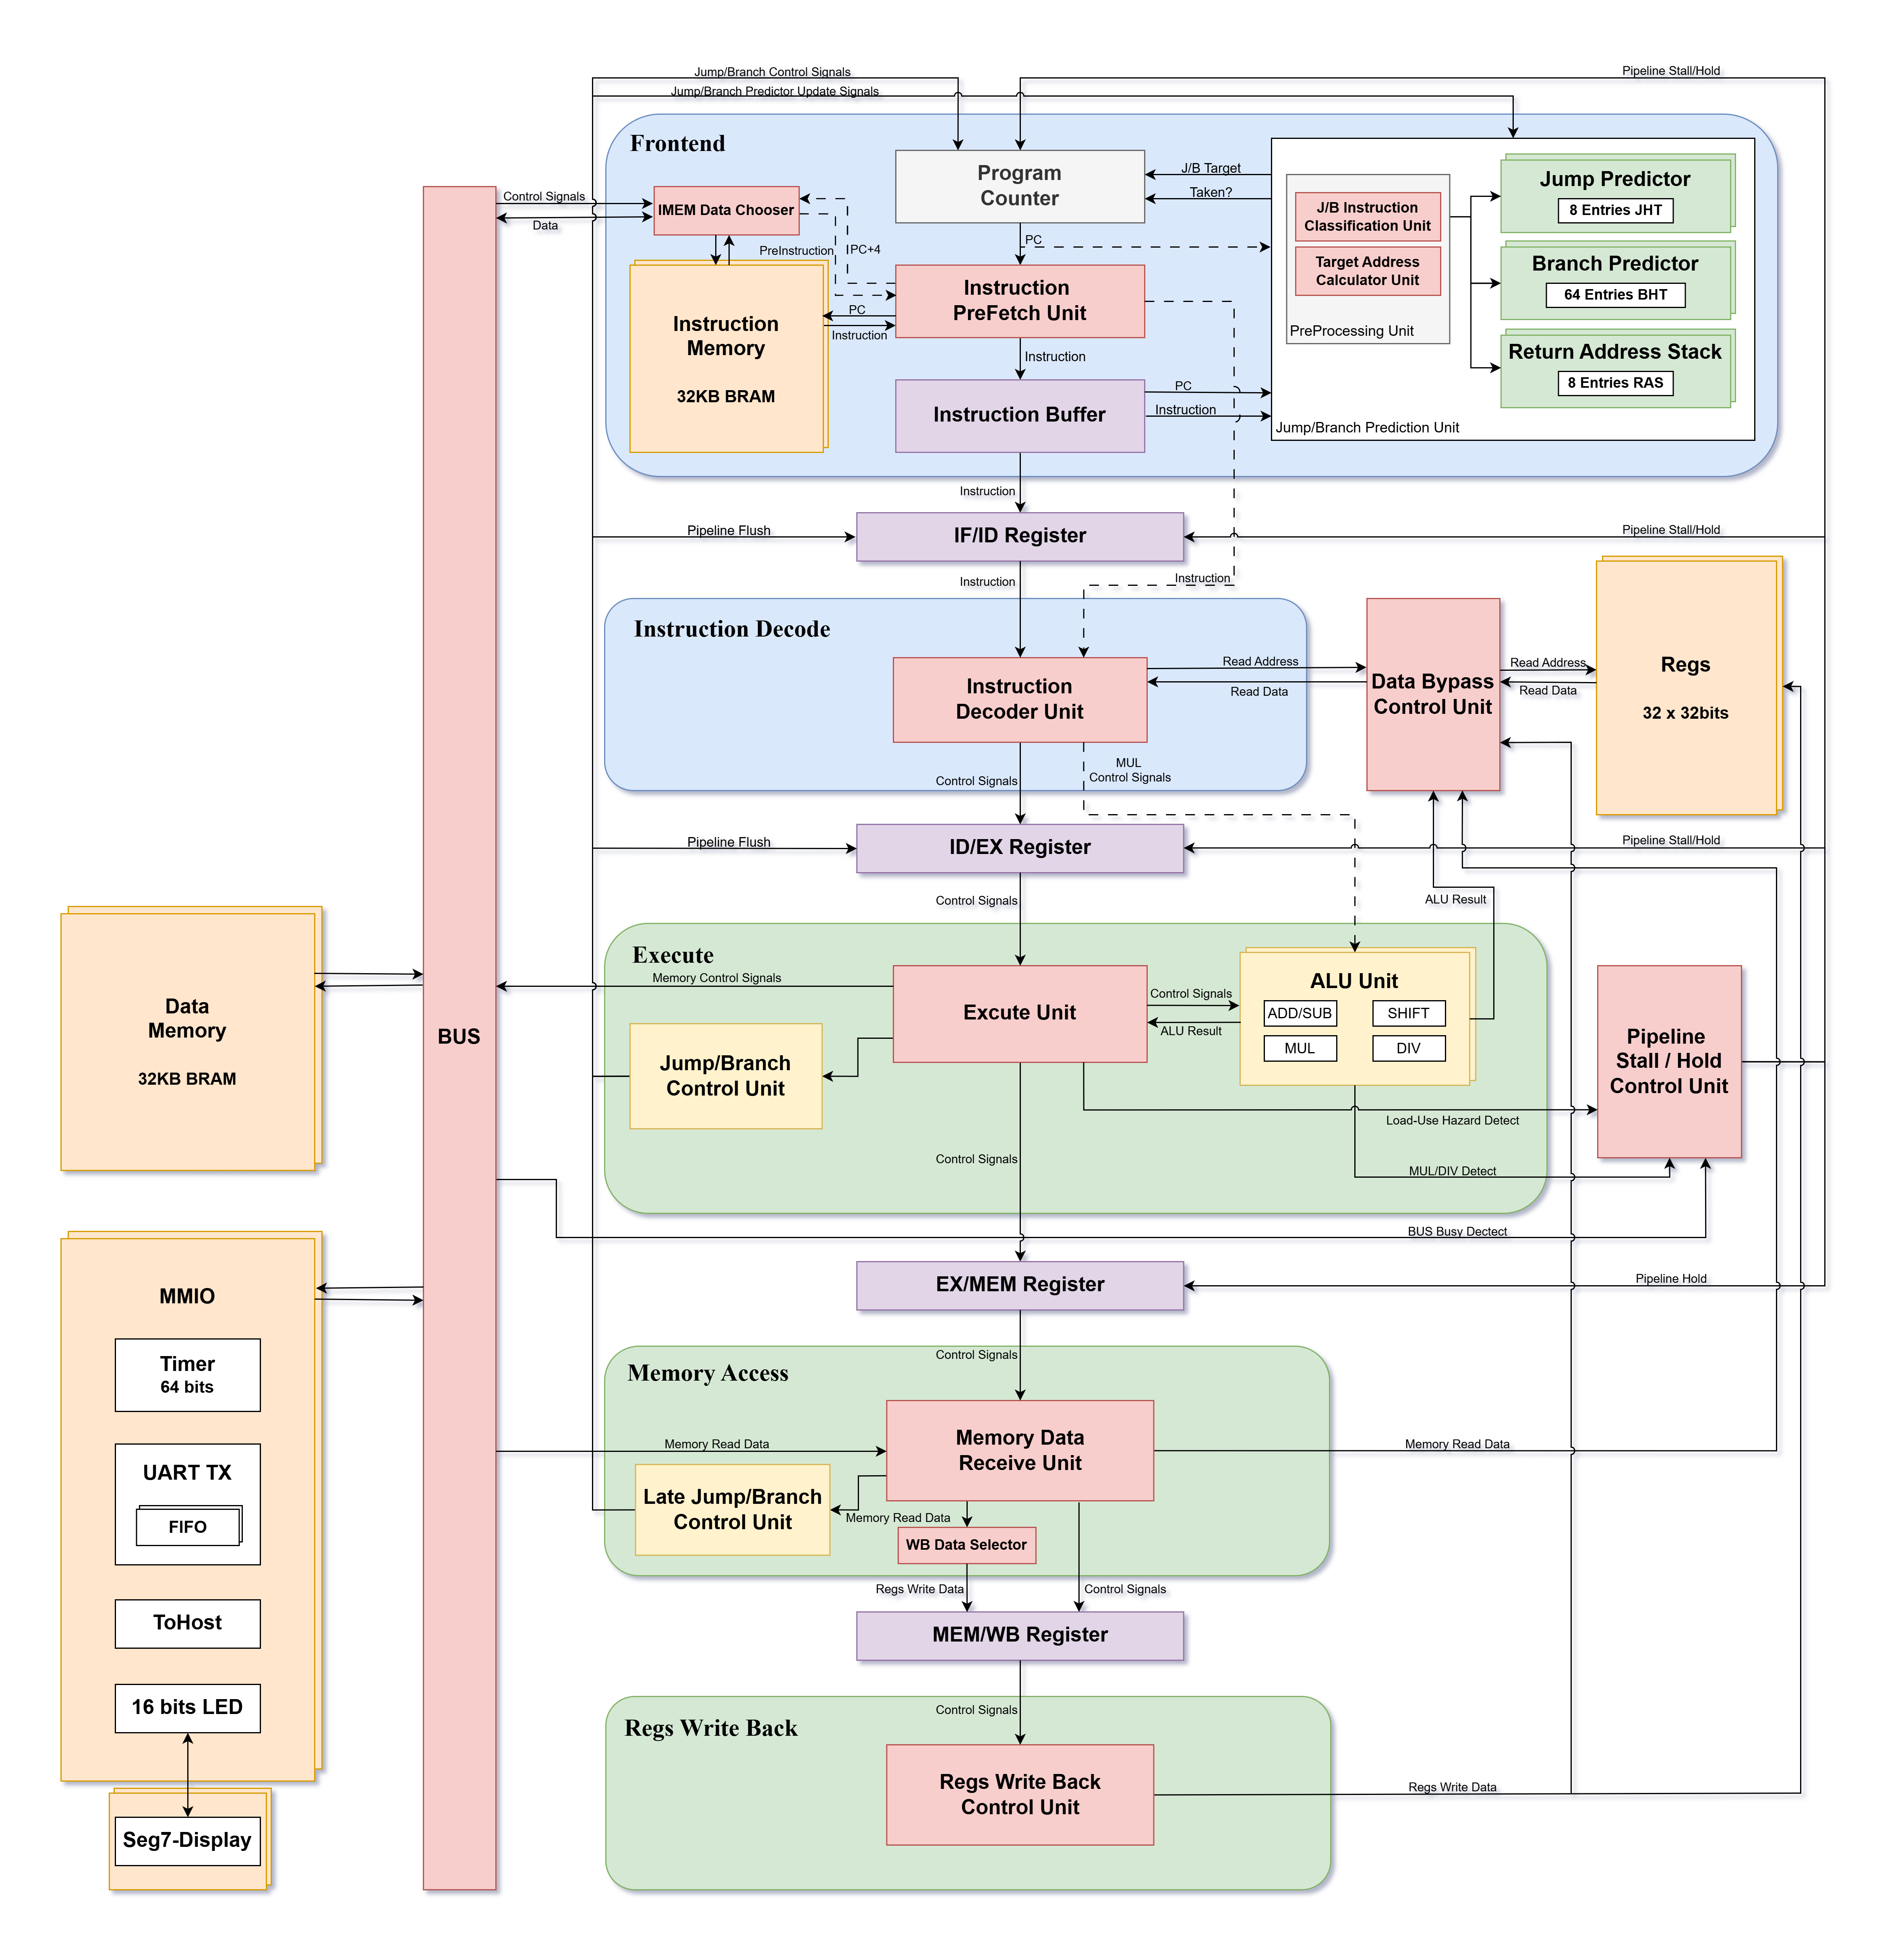
\includegraphics[
        width=\textwidth,
        height=\textheight,
        keepaspectratio
    ]{figures/sxqcpu_architecture.png}
    \caption{CPU 总体架构图}
\end{figure}

\subsection{总体能力}
\paragraph{当前版本支持指令类别}
    当前处理器面向 \texttt{RV32IM} 指令集实现，译码逻辑覆盖RV32I基础整数计算、访存、控制转移以及 M 扩展指令(表~\ref{tab:supported_instructions})。面向裸机场景，未实现特权级、异常/中断、CSR 访问、虚拟内存等系统级机制，相关系统或同步类指令不作为有效功能路径实现。访存侧也暂时未实现非对齐访问异常，因此软件应按自然对齐方式访问半字和字数据。后续将进一步扩充支持指令并完善相关机制。

    \begin{table}[H]
      \centering
      \caption{已支持指令类别}
      \label{tab:supported_instructions}
      \begin{tabularx}{\textwidth}{lX}
          \toprule
          指令类别 & 指令集合 \\
          \midrule
          U 型立即数指令
          & \texttt{LUI}, \texttt{AUIPC} \\

          R 型整数运算
          & \texttt{ADD}, \texttt{SUB}, \texttt{SLL}, \texttt{SLT}, \texttt{SLTU}, \texttt{XOR}, \texttt{SRL}, \texttt{SRA}, \texttt{OR}, \texttt{AND}
  \\

          I 型整数运算
          & \texttt{ADDI}, \texttt{SLTI}, \texttt{SLTIU}, \texttt{XORI}, \texttt{ORI}, \texttt{ANDI}, \texttt{SLLI}, \texttt{SRLI}, \texttt{SRAI} \\

          控制转移指令
          & \texttt{JAL}, \texttt{JALR}, \texttt{BEQ}, \texttt{BNE}, \texttt{BLT}, \texttt{BGE}, \texttt{BLTU}, \texttt{BGEU} \\

          访存指令
          & \texttt{LB}, \texttt{LH}, \texttt{LW}, \texttt{LBU}, \texttt{LHU}, \texttt{SB}, \texttt{SH}, \texttt{SW} \\

          M 扩展乘法指令
          & \texttt{MUL}, \texttt{MULH}, \texttt{MULHSU}, \texttt{MULHU} \\

          M 扩展除法指令
          & \texttt{DIV}, \texttt{DIVU}, \texttt{REM}, \texttt{REMU} \\
          \bottomrule
      \end{tabularx}
  \end{table}

\paragraph{存储访问与 MMIO 范围}
    本设计采用独立的指令存储器、数据存储器与 MMIO 外设地址空间。IMEM 与 DMEM 均使用片上 BRAM 实现，当前容量均为 \texttt{32KiB}。地址划分如表~\ref{tab:mem_map} 所示，MMIO 寄存器映射如表~\ref{tab:mmio_map} 所示。具备一条基于Wishbone协议的总线，用于连接各类设备。

    \begin{table}[H]
        \centering
        \caption{存储地址空间划分}
        \label{tab:mem_map}
        \begin{tabularx}{\textwidth}{lllX}
            \toprule
            区域 & 基地址 & 地址范围 & 说明 \\
            \midrule
            IMEM
            & \texttt{0x00000000}
            & \texttt{0x00000000--0x00007FFF}
            & 指令存储器，\texttt{8192} 个 32 位字（32KB），由 \texttt{imem.mem} 初始化 \\

            DMEM
            & \texttt{0x00010000}
            & \texttt{0x00010000--0x00017FFF}
            & 数据存储器，\texttt{8192} 个 32 位字（32KB），支持字节、半字、字访问 \\

            MMIO
            & \texttt{0xF0000000}
            & \texttt{0xF0000000--0xF000003F}
            & 外设寄存器区域，高 4 位为 \texttt{0xF}，低 6 位作为寄存器偏移 \\
            \bottomrule
        \end{tabularx}
    \end{table}

    \begin{table}[H]
      \centering
      \caption{MMIO 寄存器映射}
      \label{tab:mmio_map}
      \begin{tabularx}{\textwidth}{lllX}
          \toprule
          地址 & 偏移 & 访问属性 & 功能说明 \\
          \midrule
          \texttt{0xF0000000}
          & \texttt{0x00}
          & RO
          & \texttt{TIMER\_LO}：64 位周期计数器低 32 位 \\

          \texttt{0xF0000004}
          & \texttt{0x04}
          & RO
          & \texttt{TIMER\_HI}：64 位周期计数器高 32 位 \\

          \texttt{0xF0000008}
          & \texttt{0x08}
          & WO
          & \texttt{TOHOST}：程序完成标志，写入 bit0 为 1 表示程序结束 \\

          \texttt{0xF000000C}
          & \texttt{0x0C}
          & WO
          & \texttt{LED}：驱动 FPGA 板上 16 位 LED \\

          \texttt{0xF0000010}
          & \texttt{0x10}
          & WO
          & \texttt{UART\_TX}：发送数据寄存器，写入低 8 位进入发送队列 \\

          \texttt{0xF0000014}
          & \texttt{0x14}
          & RO
          & \texttt{UART\_STATUS}：UART状态寄存器 \\
          \bottomrule
      \end{tabularx}
  \end{table}
\subsection{前端架构与前端架构创新机制}
\subsubsection{动态压缩前端机制}
\paragraph{动态压缩前端机制的引入背景}
    对于标准五级流水线架构，当指令运行出现控制冲突时，往往用冲刷流水线（Pipeline Flush）的方式来解决冲突。然而，每次Flush都必然将2条跳转分支指令的后续指令无效化，须于两个周期之后方有指令重新进入EX阶段，最终会致使两个周期的浪费。\\
    因而，较为高性能的处理器一般都会引入跳转分支预测机制，通过此机制，当指令进入IF阶段时便开始判断是否要发生跳转/要跳转到哪个地址，从而使跳转分支指令与目标指令“无缝衔接”，节省下来Flush的2个周期。（图~\ref{fig:5stagepipelineflushandbp}）
    \begin{figure}[H]
        \centering
        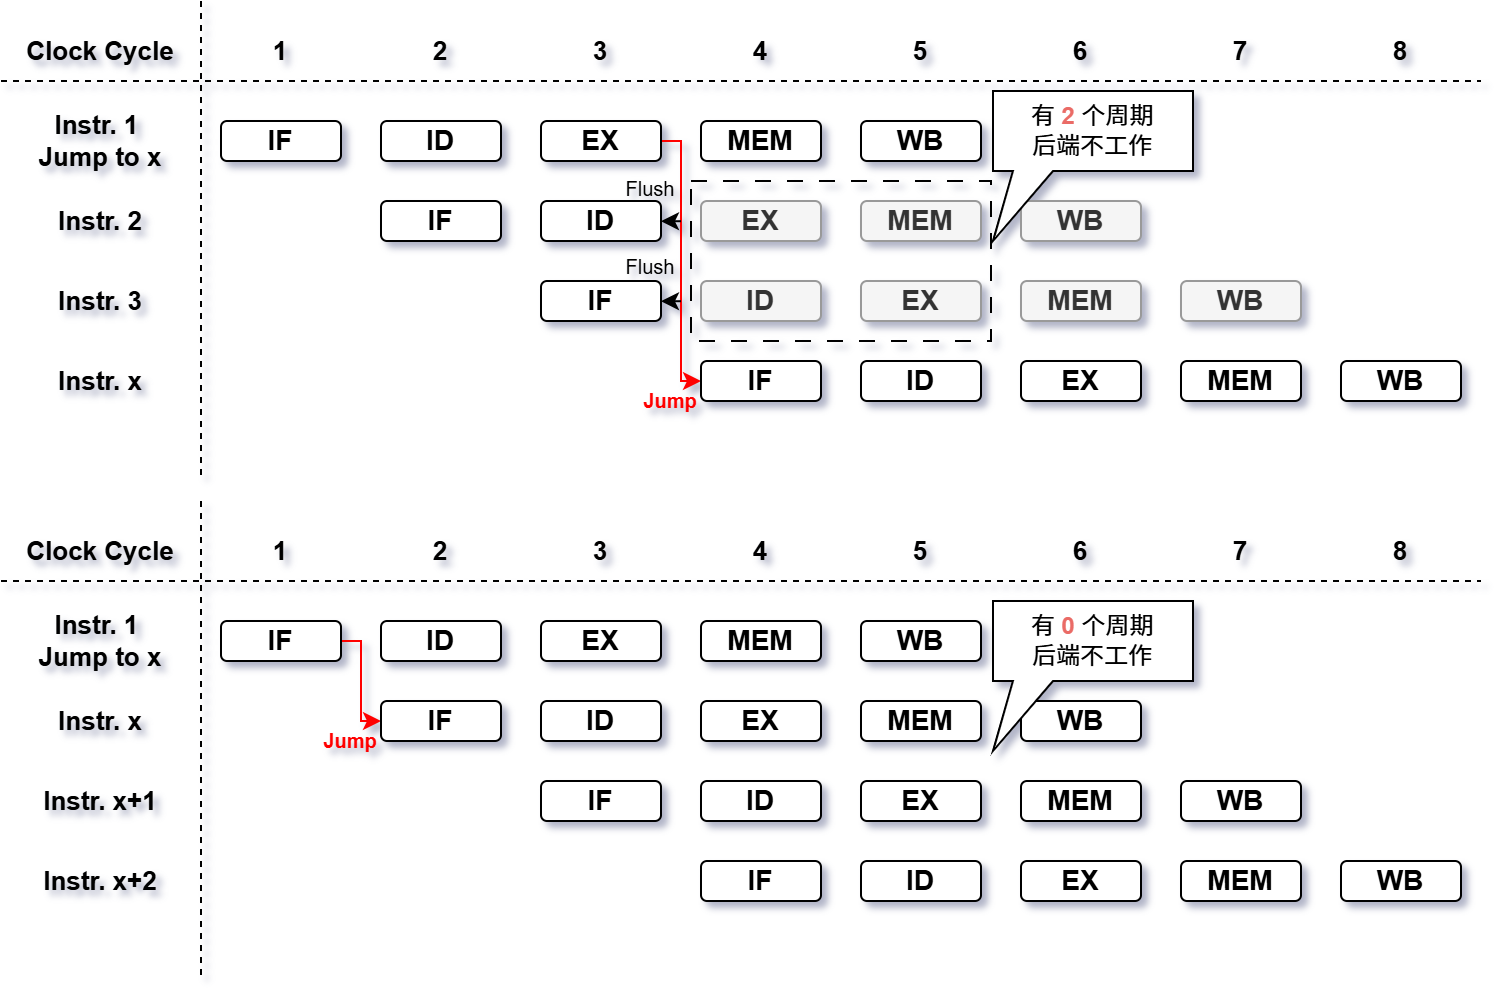
\includegraphics[width=0.9\linewidth]{figures/pipeline_flush_branch_prediction.png}
        \caption{标准五级流水线的跳转分支Flush机制与跳转分支预测机制流水线示意图}
        \label{fig:5stagepipelineflushandbp}
    \end{figure}
    常用跳转分支预测有静态预测All Taken、BTFNT，动态预测Bimodal BP、PAp、PAg、GAp、GAg、GSELECT、GSHARE、TAGE等多种实现方法，然而，其绝大部分高性能实现均需要构建维护较大数据表，如BTB、BHT、PHT、GHT等，使得资源消耗与功率消耗翻倍。而之所以其涉及资源较多，又往往是因为需要记录完整跳转地址，或是为缓解仅用PC或PC与历史模式哈希得到索引导致的别名问题。因而，若可以用低资源消耗的其他方式轻易得知跳转分支目标地址，并且引入更多信息加入索引哈希，便可以在低资源消耗的情况下，获得更好的跳转分支预测准确率。\\
    最好的方法其实便是在跳转分支预测的周期（即指令的IF阶段）就取得指令本身，并将指令本身加入预测，因为指令本身便隐含了指令类型、跳转分支偏置、比较寄存器等多种信息。但是，由于该设计使用Dual Port BRAM实现IMEM，故读IMEM至少会有1拍的固定延迟。对于本设计最开始的五级流水线版本设计来说，只能在IF的当拍将访问地址输入IMEM，并在下一拍拿到指令（为省下周期，本设计IMEM访问时不停止流水线，直接将这一拍当成等同于IF/ID寄存器的一拍来使用，将第IF+1周期得到的指令直传ID），从而错过IF阶段的跳转分支预测。（图~\ref{fig:5stagepipelineinstructionfetch}）
\begin{figure}[H]
    \centering
    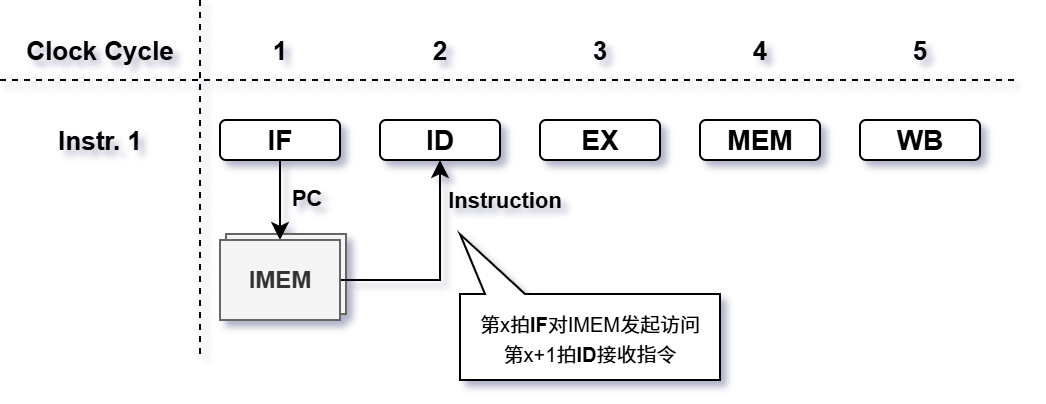
\includegraphics[width=0.6\linewidth]{figures/five_stage_instruction_fetch.png}
    \caption{五级流水线下的取指过程示意图}
    \label{fig:5stagepipelineinstructionfetch}
\end{figure}
为解决此问题，一个方案是让取指过程可以在1个周期内完成，典型实现便是使用LUTRAM构建一个ICache，即指令缓存。然而，ICache逻辑复杂，且需要将指令总线支持位宽扩充，将会引入更多资源消耗。并且LUTRAM读取也具有较长的时序路径，极有可能在100MHz下导致时序违例。\\另一个方案则是加深一级流水线，在IF级之前加入一级PreIF（Pre-Instruction-Fetch），将访问IMEM移至PreIF阶段，IF则负责接收IMEM吐出的指令。采取这种方法可以基本保持资源使用不变，并大大缩短所需时序路径。但加深流水，必然意味着跳转分支预测的代价变大了，将会从原先五级流水线的Flush 2拍变成Flush 3拍（图~\ref{fig:6stagepipelineandflush}），在减少周期损失上不一定合算。因此，本设计创新设计并使用了\textbf{\textit{动态前端压缩机制}}，使得在确保跳转分支预测可以具备指令本身的信息的同时，保持资源消耗基本不变，并使Flush代价与标准五级流水线无异。
\begin{figure}[H]
    \centering
    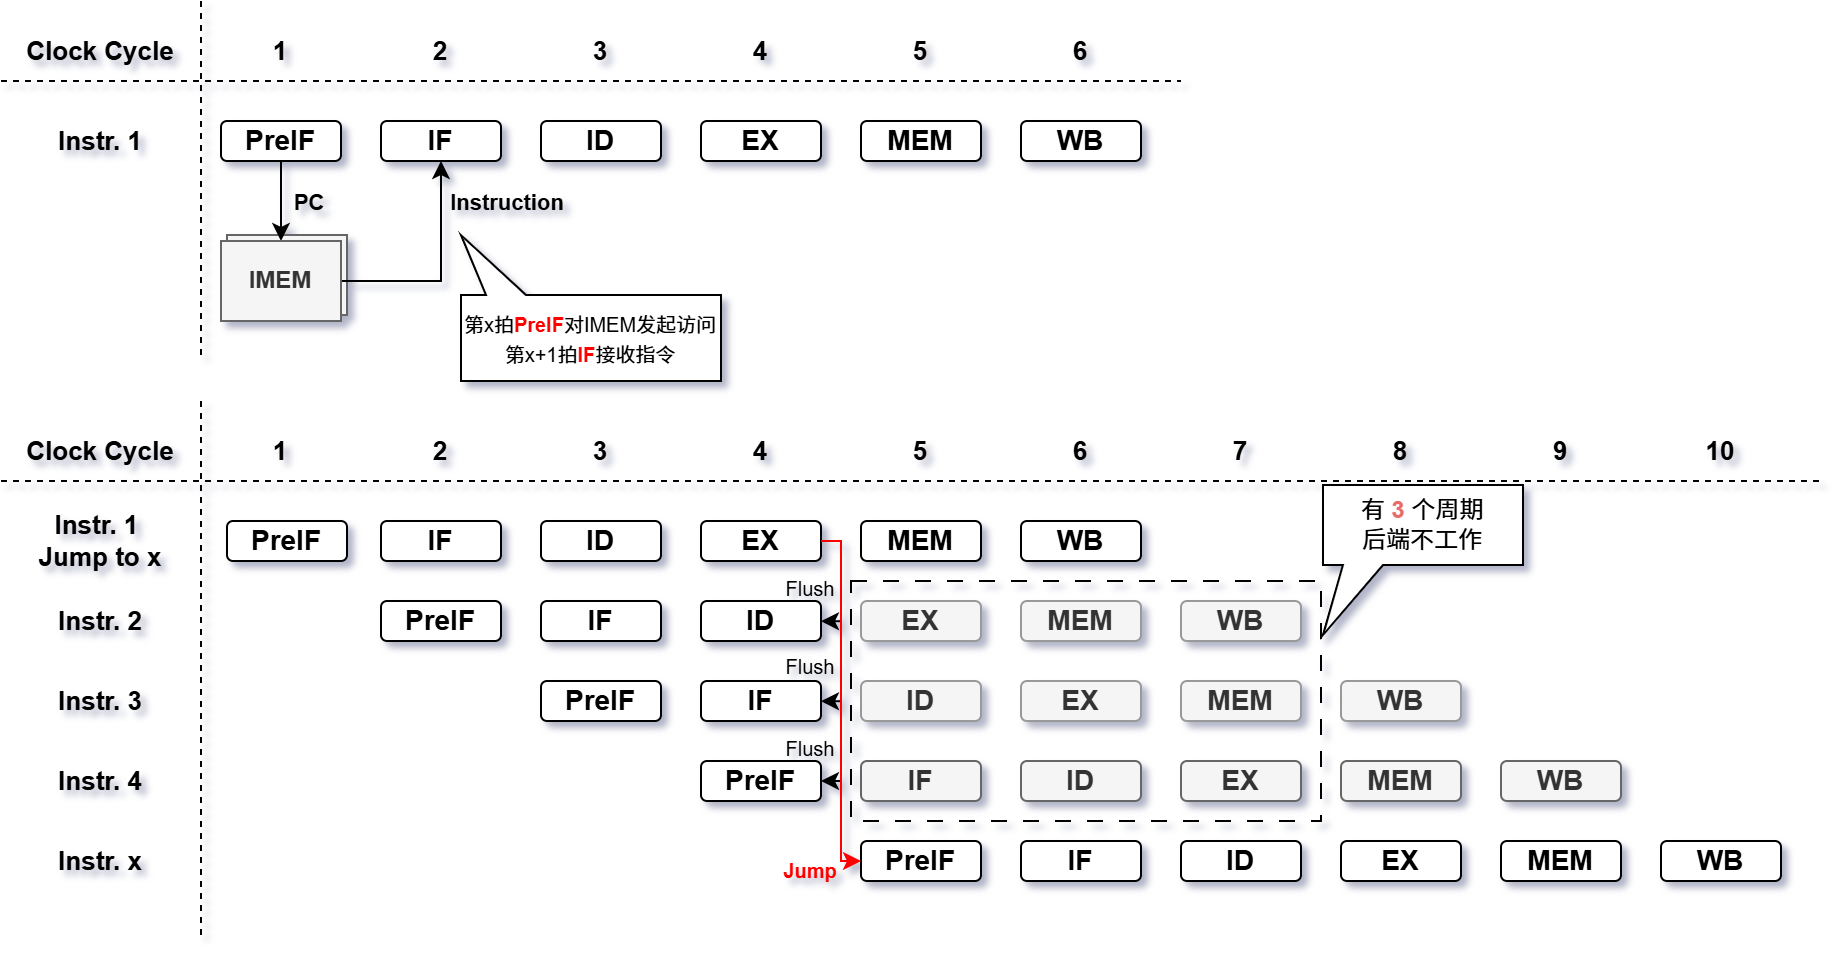
\includegraphics[width=0.97\linewidth]{figures/six_stage_instruction_fetch_flush.png}
    \caption{六级流水线下的取指过程与跳转分支Flush机制示意图}
    \label{fig:6stagepipelineandflush}
\end{figure}
\paragraph{动态压缩前端机制}
为解决上述问题，本设计创新设计并使用动态前端压缩机制，使流水线深度可以在五、六级间视条件动态调节。一般情形时，流水线为六级流水线，完成PreIF - IF - ID - EX - MEM - WB，其中IF阶段进行跳转分支预测。而当程序从头开始运行，或发生跳转（包含标准情形EX阶段引发的跳转、跳转分支预测提前引发的跳转、预测错误导致EX阶段发生的重定向跳转）时，调节相关控制信号，使得流水线前端由PreIF - IF - ID压缩为PreIF - ID，退变为五级流水线，即PreIF访问IMEM的下一拍，IMEM吐出的指令直接跳过IF转发给ID阶段。\\同时，为了减少因为缺少IF阶段而不能结合指令本身进行分支预测的指令数，当发生前端压缩的时候，需要利用BRAM的双口特性，同时使用IMEM的32位宽取指端口和32位宽读数据端口，一次性读出两条指令，即本条触发前端压缩的指令以及本条指令的下一条正常非压缩指令。（图~\ref{fig:dynamicstagesnumberpipeline}）
\begin{figure}[H]
    \centering
    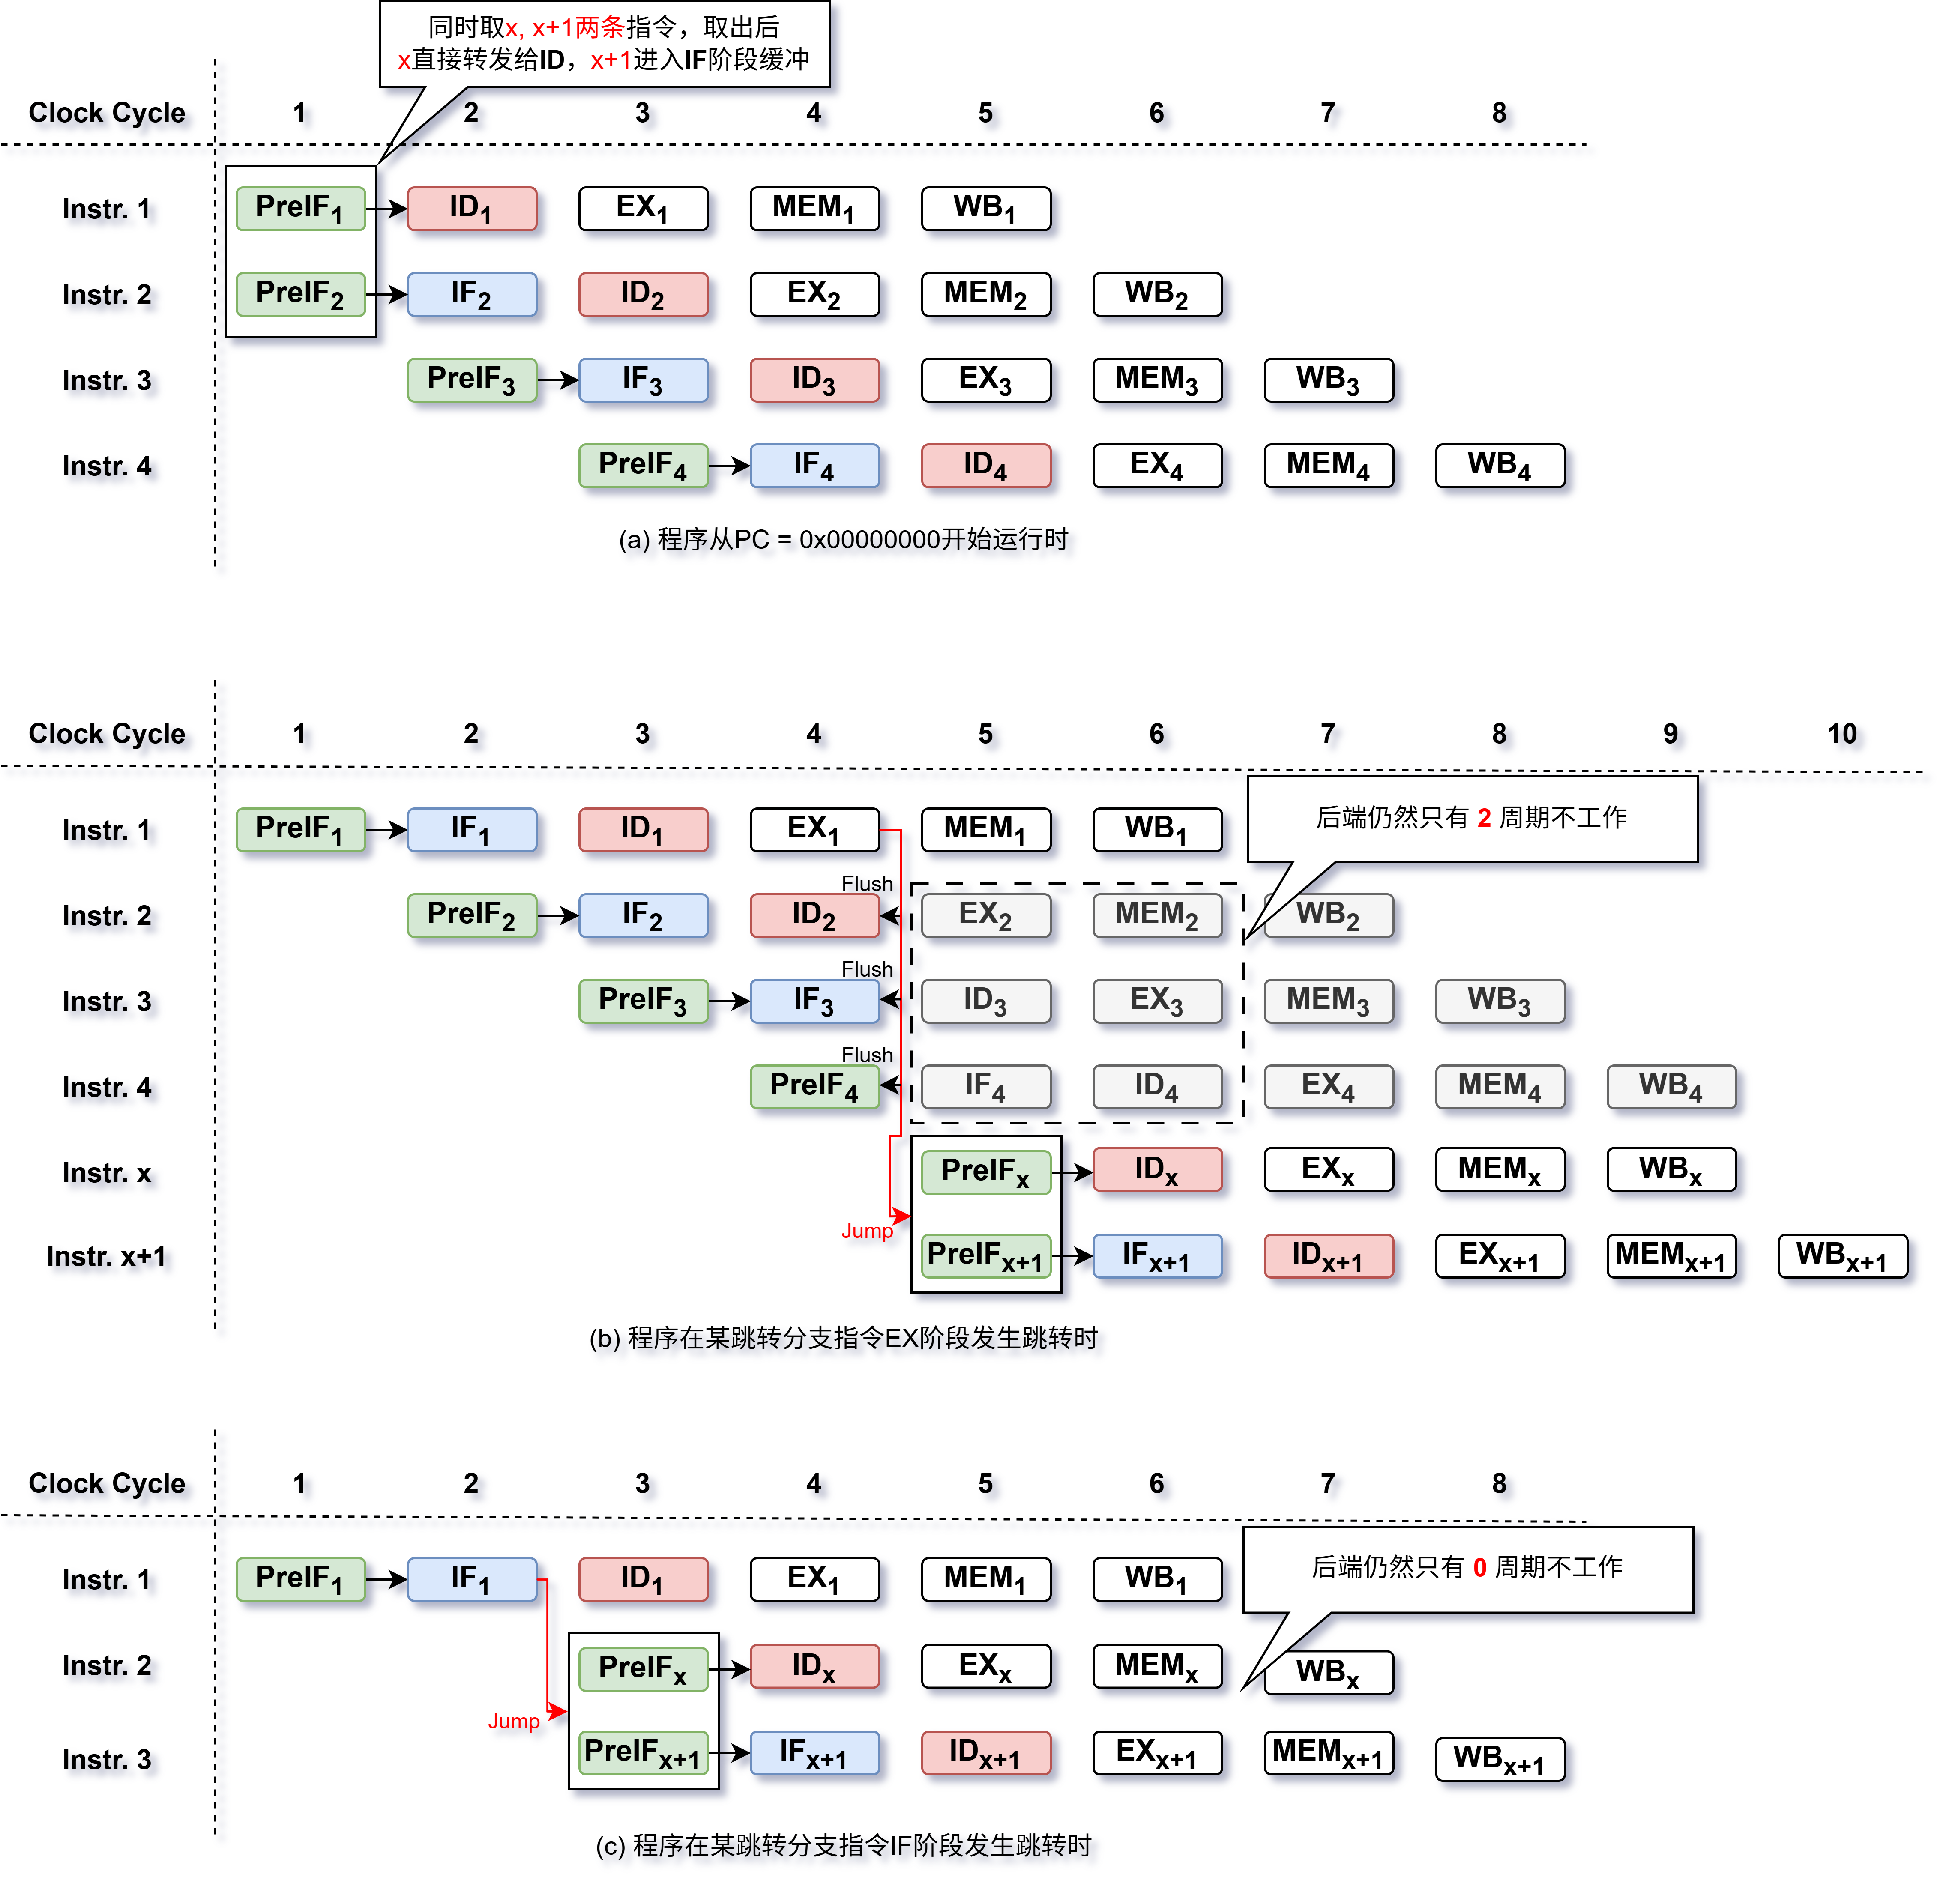
\includegraphics[width=0.97\linewidth]{figures/dynamic_frontend_compression.png}
    \caption{动态前端压缩流水线示意}
    \label{fig:dynamicstagesnumberpipeline}
\end{figure}
可以发现，通过结合了加深流水线与条件双取指两种机制的动态压缩前端机制，成功使得在不引入复杂Cache机制、最小新增逻辑、最小新增资源消耗的前提下，IF阶段的跳转分支预测可以拿到指令本身的信息，同时不增加任何多余的Flush等周期损耗。为接下来的特殊设计的跳转分支预测打下基础。

\subsubsection{特殊设计的低资源跳转分支预测机制}
\paragraph{低资源跳转分支预测机制的引入背景}
    在前文所述的动态压缩前端机制基础上，本设计能够在 IF 阶段取得指令本身，并在预测发生前获得指令类型、立即数字段与寄存器编号等信息。因此，跳转分支预测不必仅依赖 PC 或历史状态表，也可以利用指令编码中携带的结构化信息进行分类处理。\\
    对于 RISC-V 控制流指令，不同指令的方向确定性与目标地址来源并不相同。\texttt{JAL} 指令语义上恒为 Taken，目标地址由 PC 与 J 型立即数相加得到；B 型条件分支的目标地址同样由 PC 与 B 型立即数相加得到，但方向需要预测；\texttt{JALR} 的目标地址依赖寄存器值，前端无法仅凭指令字段直接得到真实目标。若使用统一的大容量 BTB 覆盖全部控制流指令，会对可直接计算目标地址的指令重复保存目标地址，并引入额外的查表、比较和目标选择路径。基于此，本设计按控制流指令的语义特征拆分预测路径：\texttt{JAL} 直接计算目标地址，B 型分支使用 Tagged BHT 预测方向，返回类 \texttt{JALR} 使用 RAS 预测目标，非返回类 \texttt{JALR} 使用小容量 JTB 缓存目标地址。\\
    \begin{table}[H]
        \centering
        \begin{tabular}{|c|c|c|}\hline
            跳转分支指令类型 & 跳转分支是否执行判断方式 & 跳转分支目标地址判断方式 \\\hline\hline
            Jump Type(\texttt{JAL}) & 全部 Taken & 直算(PC + IMM) \\\hline
            Jump Type(\texttt{JALR}) & 全部 Taken & JTB / RAS \\\hline
            Branch Type & BHT(2BC) / BTFNT & 直算(PC + IMM) \\\hline
        \end{tabular}
        \caption{跳转分支预测模式表}
    \end{table}
    这种分类预测方式将可直接确定的信息保留在组合逻辑中处理，将前端无法直接获得的信息交由小容量预测结构维护，从而在较低资源消耗和较短查找路径下获得较好的控制流预测效果。

\paragraph{低资源跳转分支预测机制概述}
    本设计的预测机制由指令分类单元、目标地址计算单元、Branch Predictor、Jump Predictor 以及 Return Address Stack 共同构成。PreIF 阶段发起对 IMEM 的访问，下一拍 IF 阶段取回对应指令；随后，前端进行轻量级预解码，首先基于 \texttt{instr[6:2]} 判断指令是否属于 Branch、\texttt{JAL} 或 \texttt{JALR}，再根据 \texttt{rd} 与 \texttt{rs1} 编号识别 Call 与 Ret。Call 由跳转指令写回寄存器是否为 \texttt{x1} 或 \texttt{x5} 判断；Ret 的判定条件为 \texttt{JALR}、\texttt{rd=x0}、\texttt{rs1=x1/x5} 且立即数为 0。\\
    分类结果作为后续预测结构的门控信号与目标地址仲裁信号：Branch 控制 BHT 查找是否有效；\texttt{JAL} 触发直接目标地址计算；Ret 选择 RAS 作为 \texttt{JALR} 目标来源；非 Ret 的 \texttt{JALR} 进入 JTB 预测路径。各模块在前端控制逻辑仲裁下决定下一拍取指地址，并在后端真实执行结果返回后完成状态更新，整体分类关系与分类单元结构分别见（图~\ref{fig:JBInstructionClassification}）（图~\ref{fig:JBInstructionClassificationUnit}）。
    \begin{figure}[H]
        \centering
        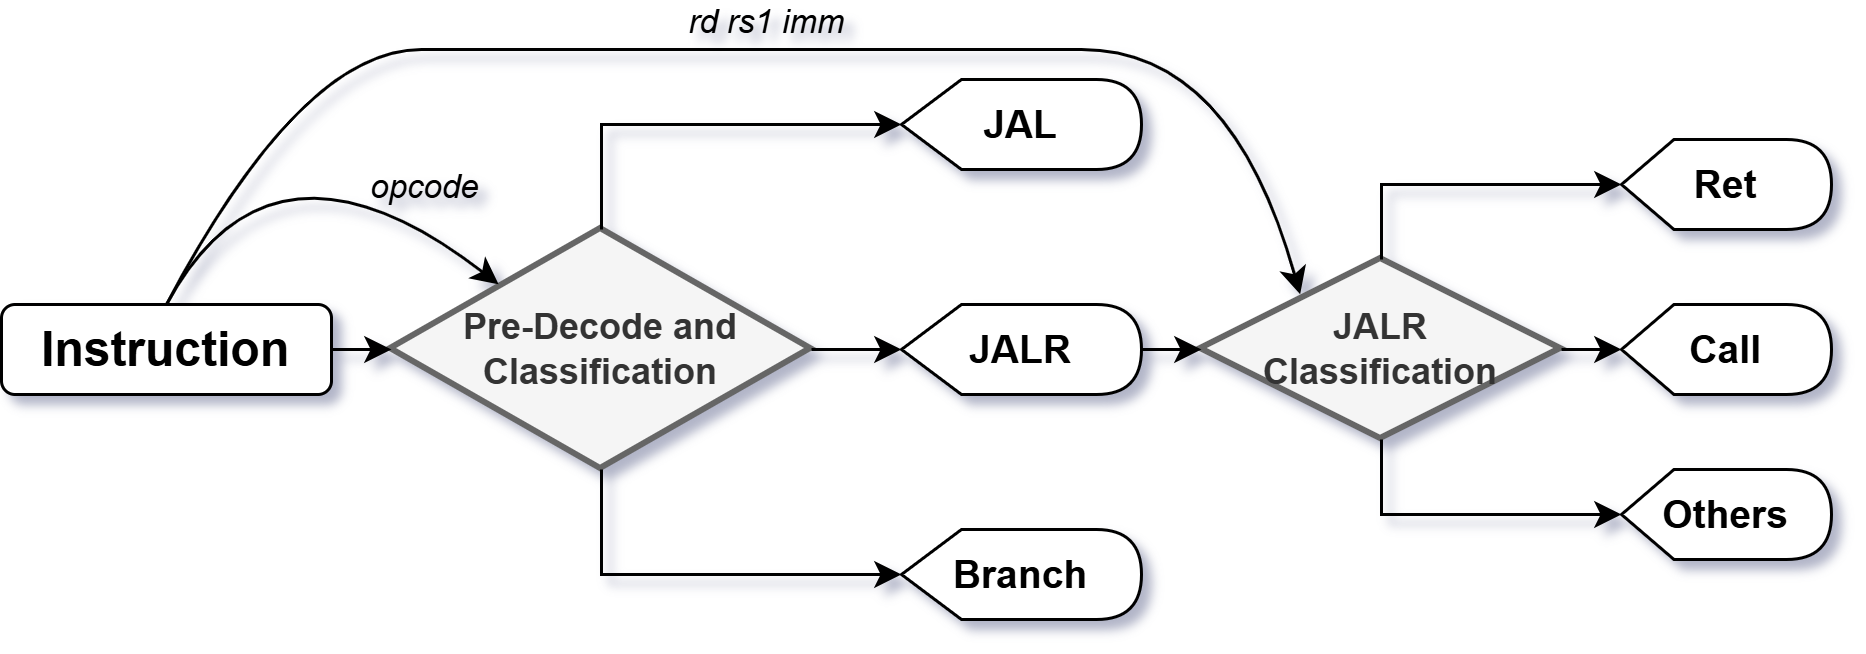
\includegraphics[width=0.6\linewidth]{figures/control_flow_instruction_classification.png}
        \caption{跳转分支指令分类示意图}
        \label{fig:JBInstructionClassification}
    \end{figure}
    \begin{figure}[H]
        \centering
        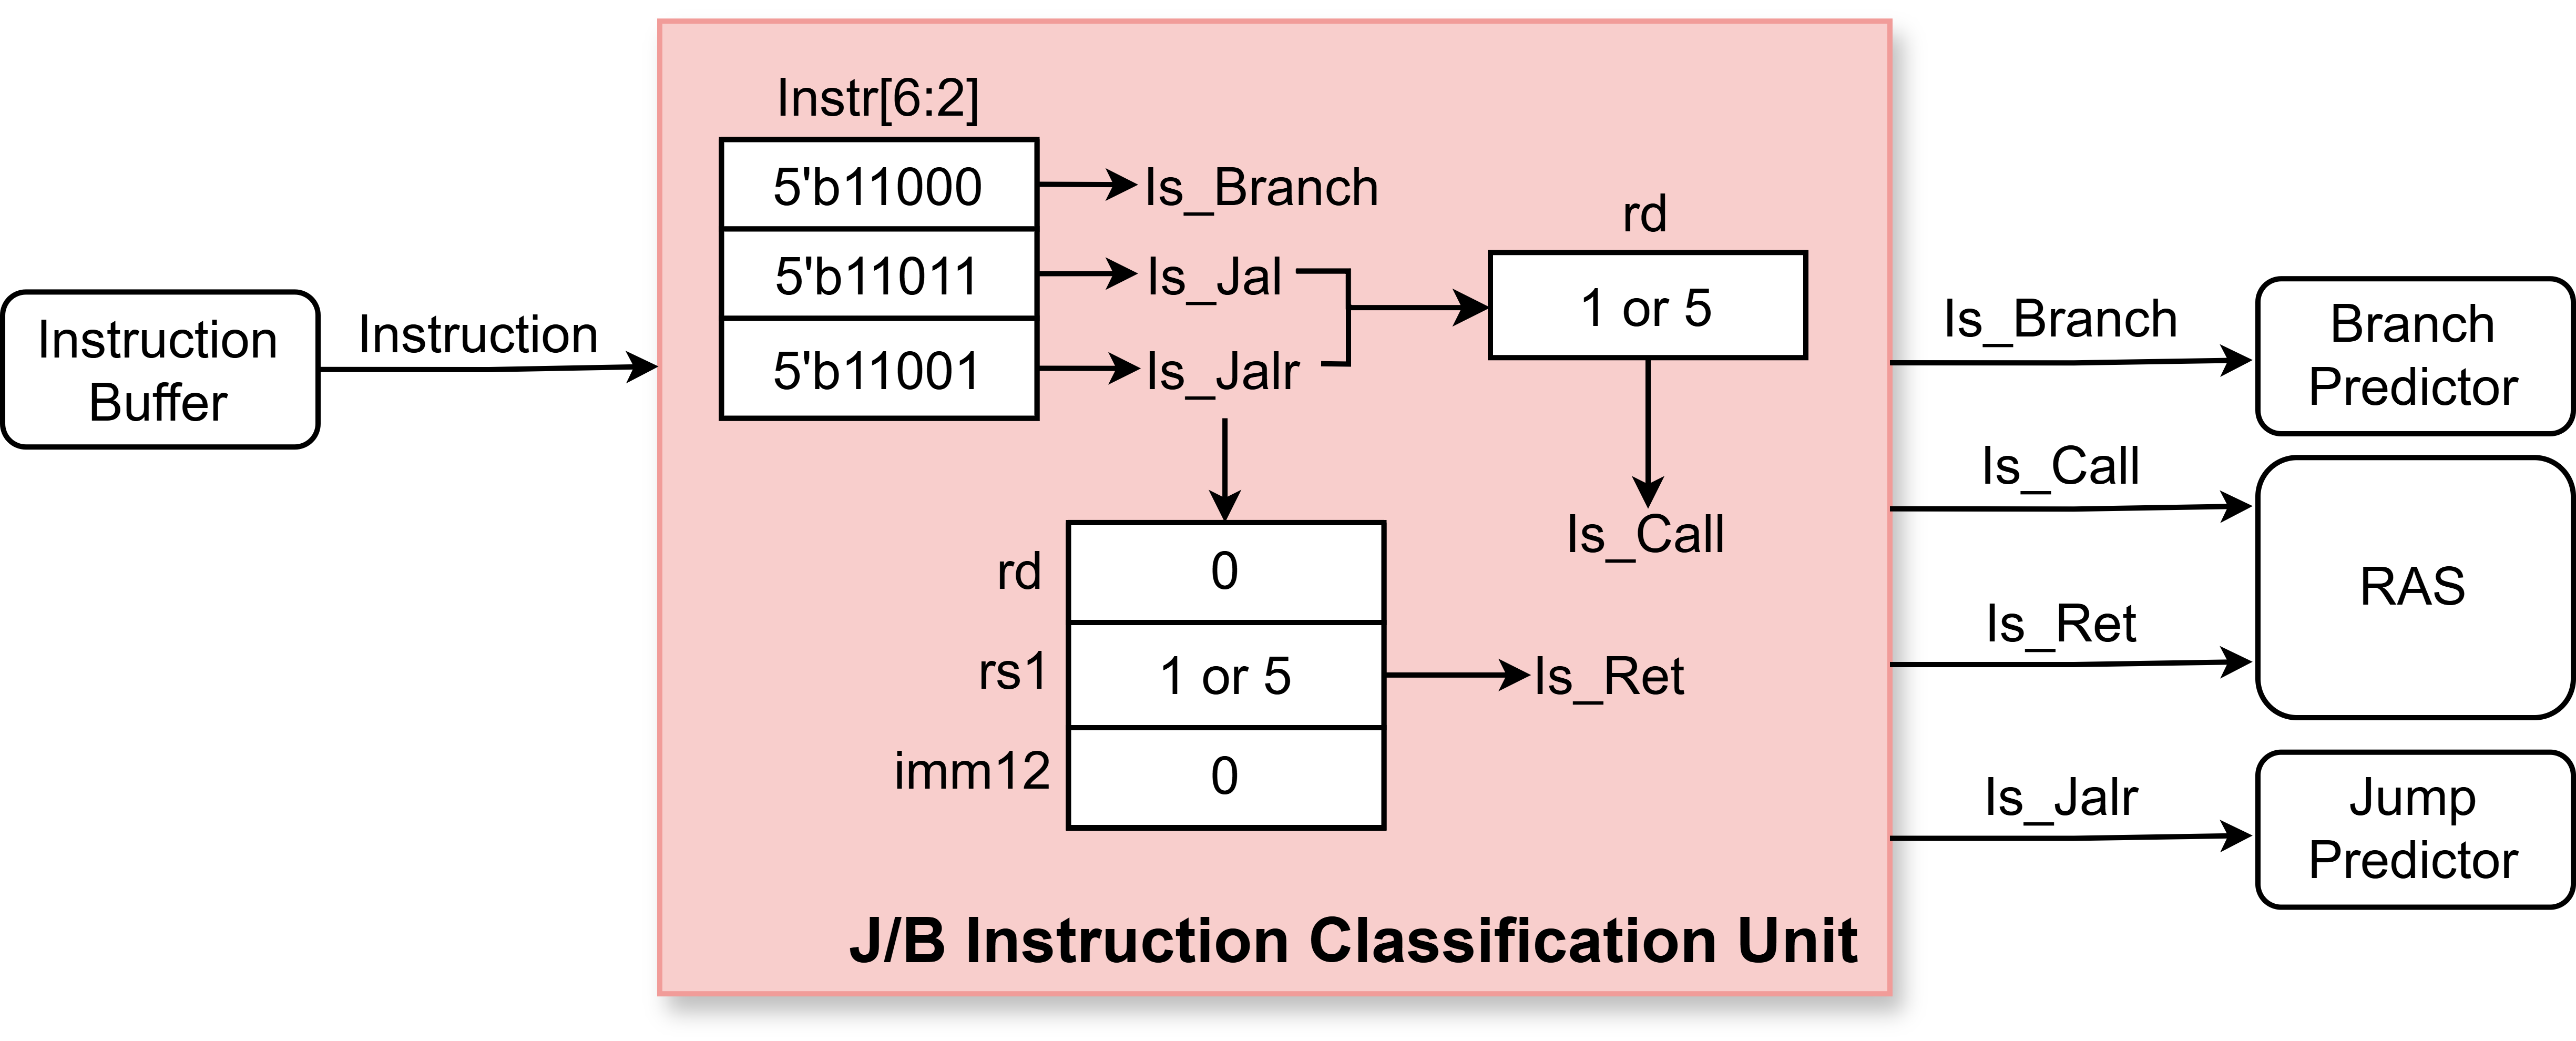
\includegraphics[width=0.7\linewidth]{figures/jb_instruction_classification_unit.png}
        \caption{跳转分支指令分类单元}
        \label{fig:JBInstructionClassificationUnit}
    \end{figure}

\subparagraph{\texttt{JAL}跳转预测}
    对于 \texttt{JAL} 指令，其方向恒为 Taken，因此无需方向预测。本设计在 IF 阶段提取 J 型立即数，并由目标地址计算单元以前端组合逻辑计算预测目标：
    \[
        target_{jal} = PC + J_{\mathrm{imm}}
    \]
    因此，\texttt{JAL} 的方向与目标均可确定性给出，不需要额外目标地址缓存。该目标地址进入前端控制逻辑，与其他可能的重定向来源共同参与下一拍取指地址仲裁。

\subparagraph{Branch分支预测}
    对于 B 型条件分支，其目标地址由 \texttt{PC + B\_imm} 决定，与寄存器值无关。因此，目标地址计算单元在前端直接生成候选目标：
    \[
        target_{br} = PC + B_{\mathrm{imm}}
    \]
    Branch Predictor 只负责方向预测，不保存分支目标地址，结构见（图~\ref{fig:Branch}）。当前实现采用 64 项 Tagged BHT，每个表项包含有效位、Tag 与 2-bit 饱和计数器。若当前指令确认为 Branch、目标表项有效且 Tag 匹配，则 BHT 命中，并使用计数器高位作为 Taken/Not Taken 预测结果；若 BHT 未命中，则采用 BTFNT 静态回退策略，即后向分支预测 Taken、前向分支预测 Not Taken。其方向预测可概括为：
    \[
        pred_{br} =
        \begin{cases}
            ctr[1], & hit_{bht}=1 \\
            B_{\mathrm{imm}}[31], & hit_{bht}=0
        \end{cases}
    \]
    为缓解小容量 BHT 的别名冲突，本设计没有直接使用 PC 低位作为唯一索引，而是将 PC 局部位段与 B 型立即数字段进行异或混合。当前 BHT 索引位宽为 6，对应 64 个表项，其索引生成过程为：
    \[
        hash[i] = PC[6+i] \oplus imm_{\mathrm{lo}}[5+i], \quad i=0,1,\cdots,5
    \]
    \[
        idx_{bht} = PC[7:2] \oplus hash
    \]
    其中 \texttt{imm\_lo[10:5]} 对应 B 型立即数字段中的局部偏移信息。该索引将 PC 低位、PC 较高局部位与分支偏移共同混合，使不同分支更均匀地映射到有限 BHT 表项中。BHT 的 Tag 由 PC 较高位形成。当前参数下，\texttt{BR\_PRED\_PC\_CANON\_BITS=12}、\texttt{BR\_PRED\_TAG\_BITS=5}，因此 Tag 实际为：
    \[
        tag_{bht} = PC[12:8]
    \]
    Tag 用于降低不同分支映射到同一索引时产生假命中的概率。更新时，若真实执行结果对应表项命中同一 Tag，则根据真实方向更新 2-bit 饱和计数器：Taken 时向强 Taken 方向递增，Not Taken 时向强 Not Taken 方向递减；若未命中，则仅在真实结果为 Taken 时分配新表项，并初始化为弱 Taken，以减少一次性 Not Taken 分支对小容量 BHT 的污染。
    \begin{figure}[H]
        \centering
        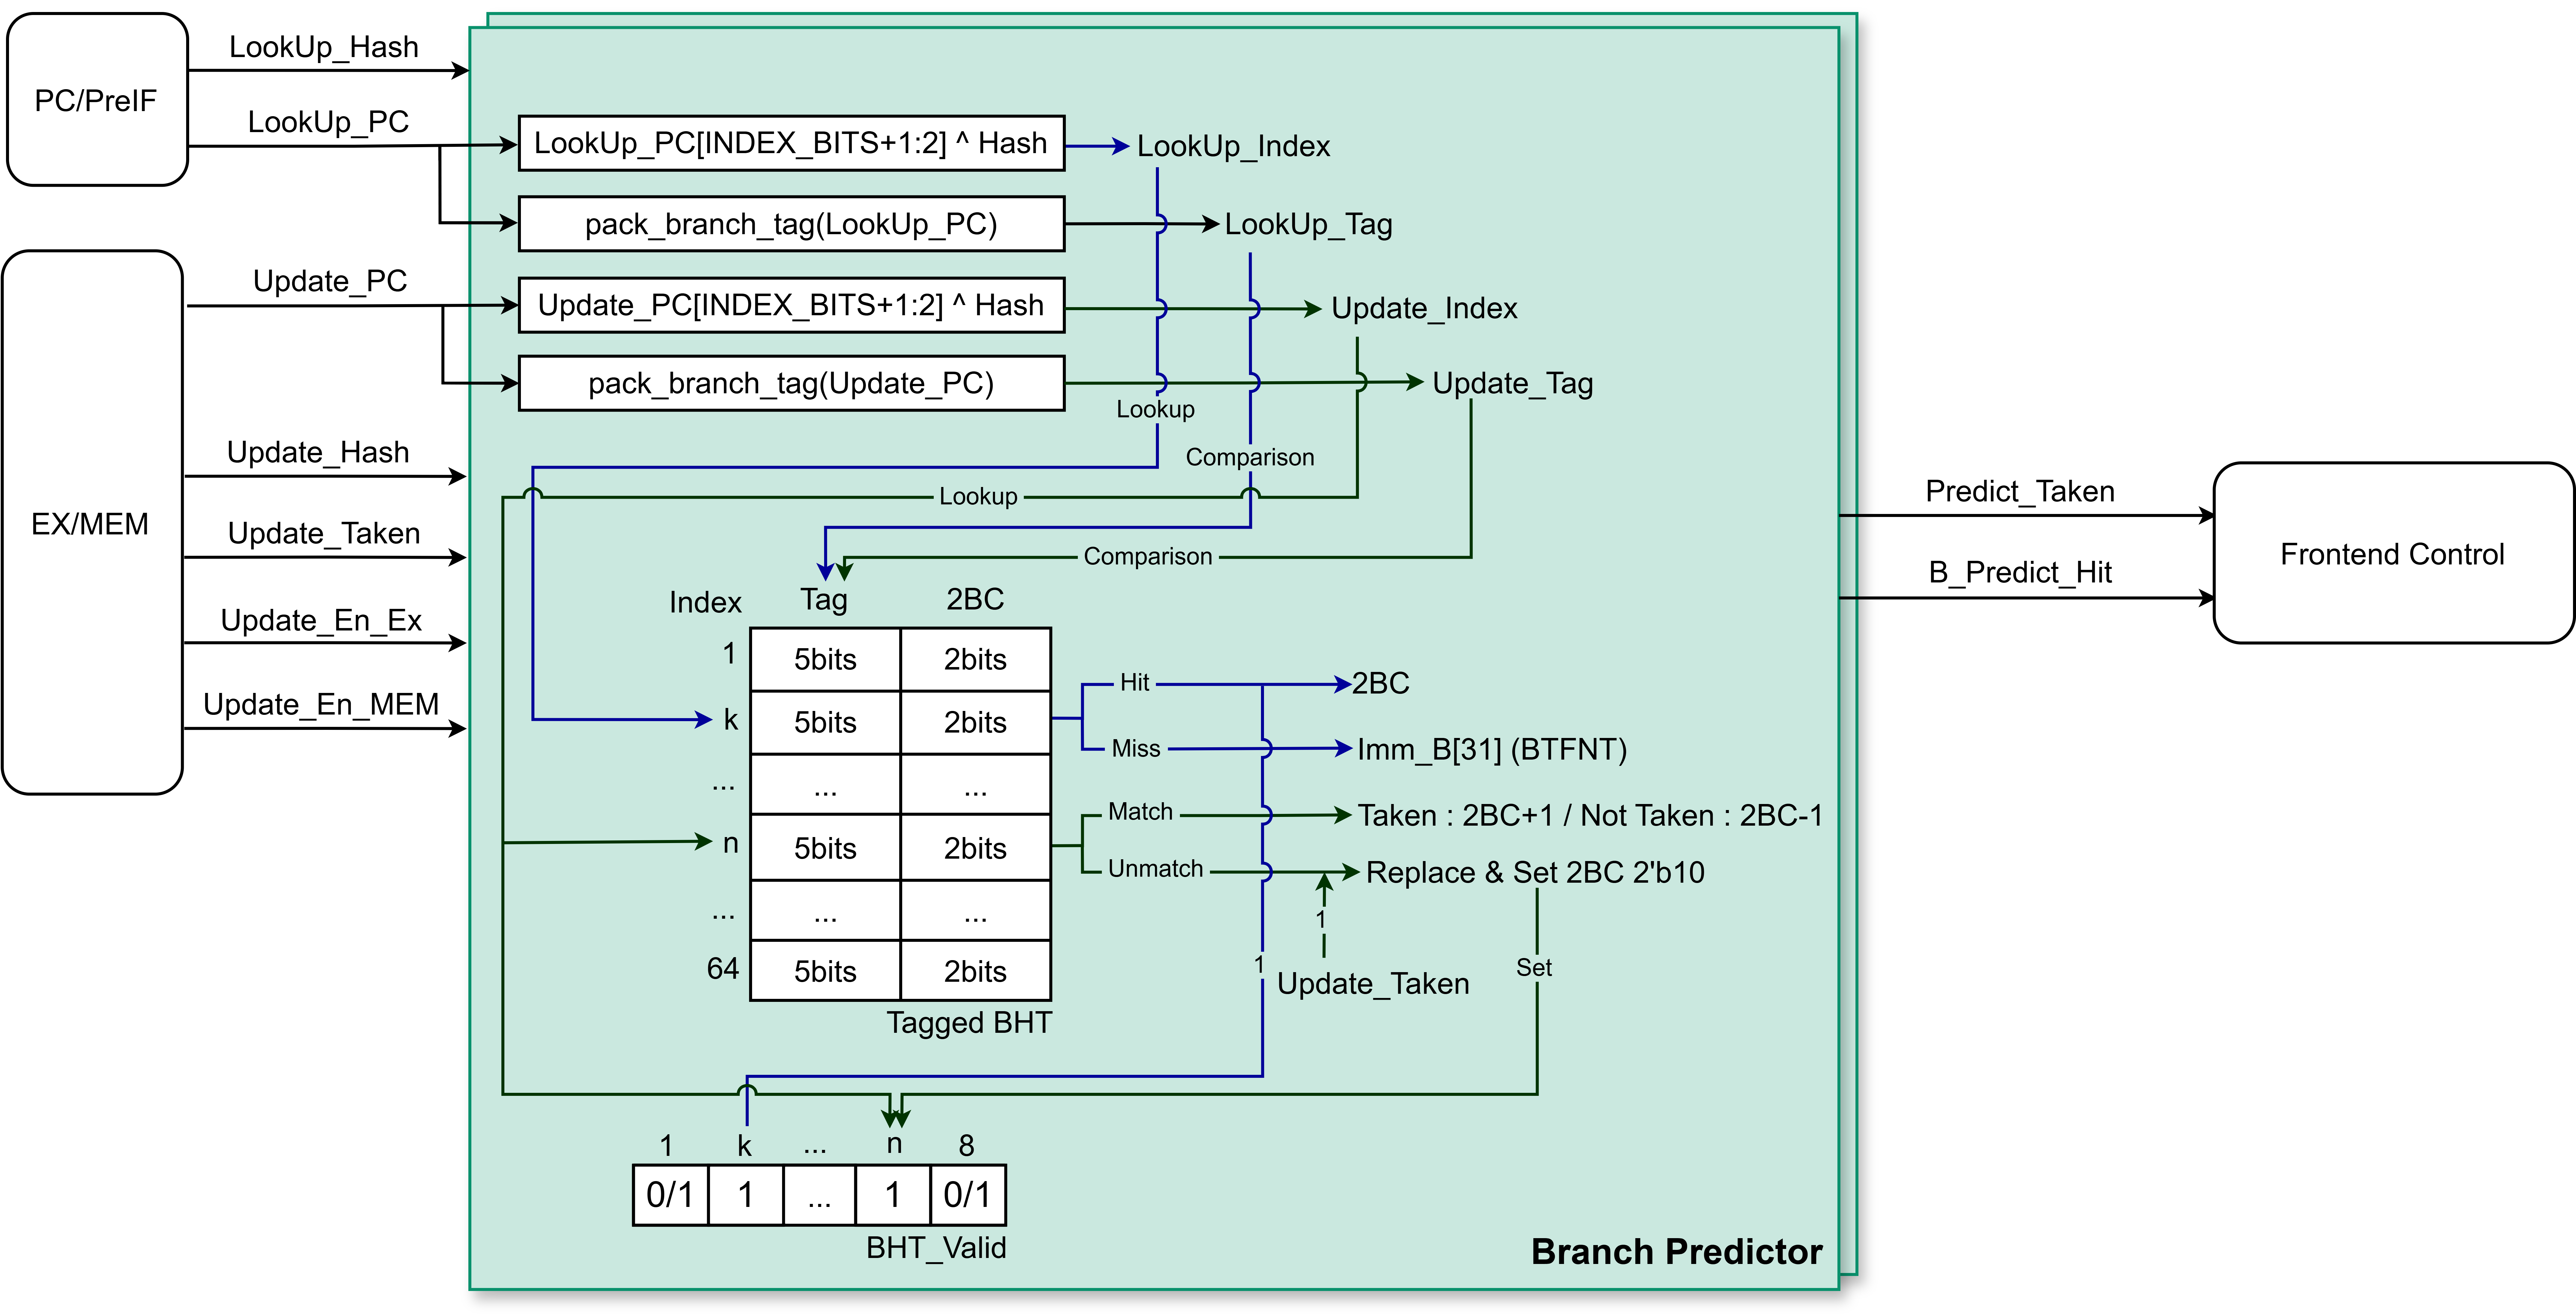
\includegraphics[width=0.9\linewidth]{figures/branch_predictor.png}
        \caption{基于BHT和BTFNT的Branch分支预测器}
        \label{fig:Branch}
    \end{figure}
\subparagraph{\texttt{JALR}跳转预测}
    对于 \texttt{JALR} 指令，其目标地址依赖寄存器值，因此目标地址计算单元不直接由立即数生成目标，而是在 RAS 与 JTB 之间选择预测来源。返回类 \texttt{JALR} 满足 \texttt{rd=x0}、\texttt{rs1=x1/x5} 且立即数为 0；若当前 \texttt{JALR} 被识别为 Ret，则使用 RAS 当前栈顶作为预测目标；若为非 Ret，则在 JTB 命中时使用 JTB 给出的历史目标地址，未命中时不提前跳转，而是等待后端解析真实目标后进行重定向恢复。
    \begin{figure}[H]
        \centering
        \includegraphics[width=1\linewidth]{figures/return_address_stack.png}
        \caption{基于返回地址栈RAS的返回类JALR跳转预测器}
        \label{fig:RAS}
    \end{figure}
    \begin{figure}[H]
        \centering
        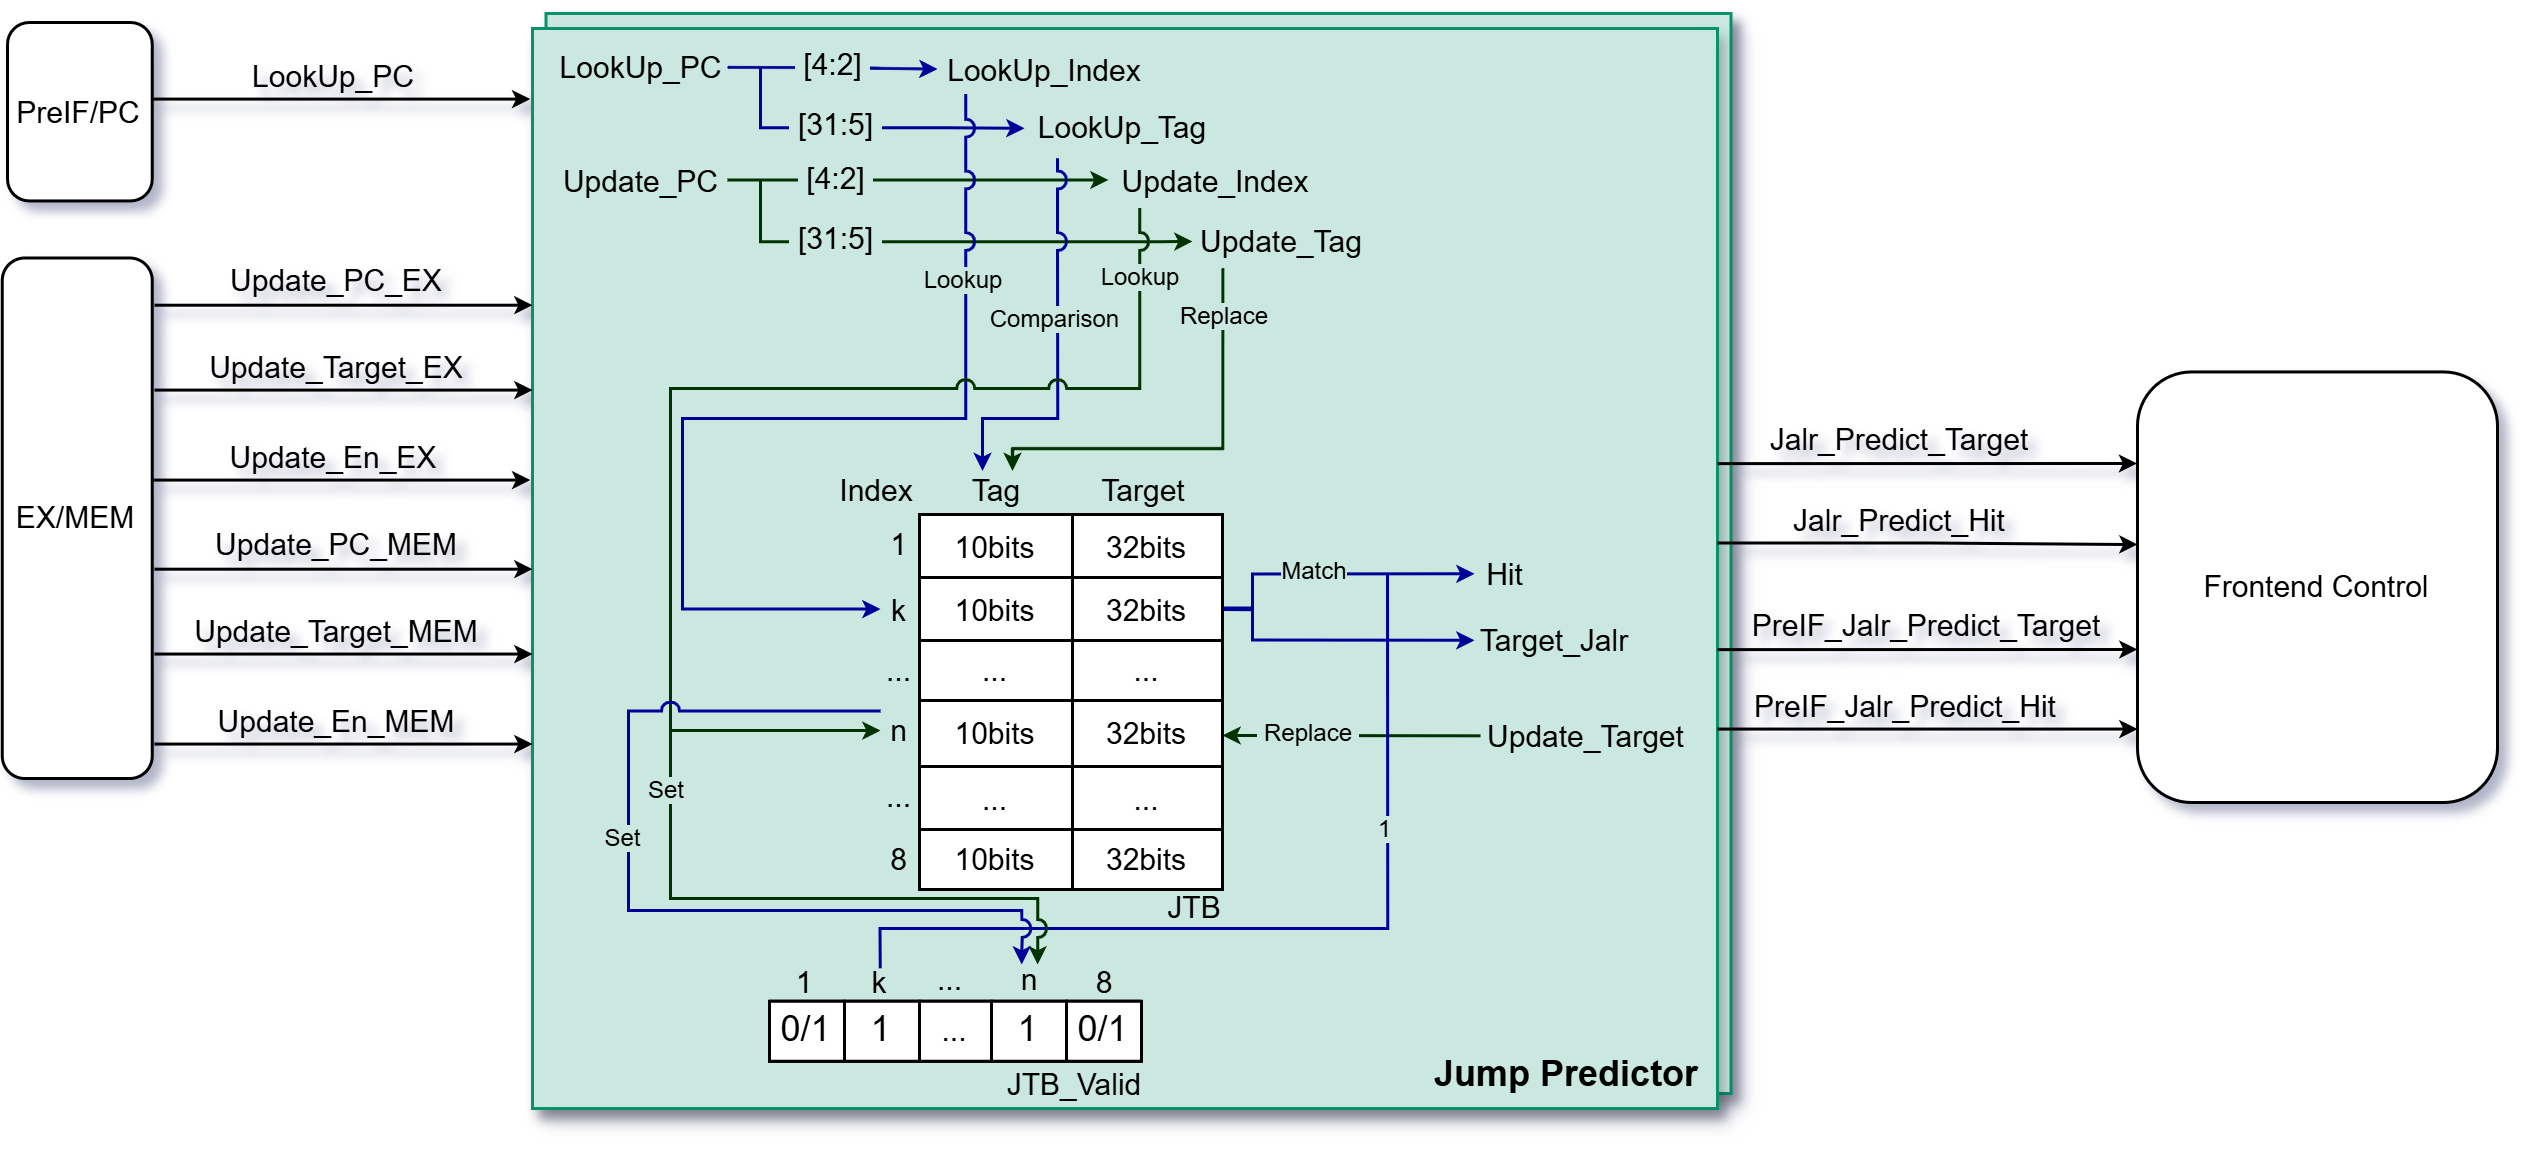
\includegraphics[width=0.9\linewidth]{figures/jump_target_buffer_predictor.png}
        \caption{普通（非返回类）JALR跳转预测器}
        \label{fig:JALR}
    \end{figure}
    Return Address Stack 用于为 Ret 指令提供低延迟目标预测，并支持动态压缩前端下的双槽位前瞻，结构见（图~\ref{fig:RAS}）。模块内部维护深度为 8 的返回地址栈及相关状态，包括 \texttt{ras\_stack}、\texttt{ras\_sp}、\texttt{ras\_count}、\texttt{ras\_top\_target\_q} 与 \texttt{ras\_next\_target\_q}。当前栈是否有效由 \texttt{ras\_count} 判断，slot0 Ret 预测直接使用当前栈顶地址。后端确认执行 Call 指令时，将返回地址 \(PC_{call}+4\) 压入 RAS；后端确认执行 Ret 指令时，从 RAS 弹出栈顶。当前端识别到 Ret 且 RAS 有效时，预测目标为：
    \[
        target_{ret} = ras\_top
    \]
    在动态压缩前端机制下，前端可能同时观察 slot0 与 slot1 两个候选指令。为避免 slot1 的返回预测受 slot0 Call/Ret 影响，RAS 生成 shadow 形式的 slot1 栈顶结果，使 slot1 基于“slot0 生效后的前瞻栈状态”进行 Ret 目标预测。若 slot0 是 Call，则 slot1 看到的栈顶等价于压入 \texttt{slot0 PC+4} 后的结果；若 slot0 是 Ret，则 slot1 看到的栈顶等价于弹出一层后的结果。该 shadow 结果只用于前端预测，不提前修改真实 RAS 状态。\\
    对于非返回类 \texttt{JALR}，Jump Predictor 采用 8 项直接映射 JTB 实现，结构见（图~\ref{fig:JALR}），每个表项包含有效位、Tag 与目标地址。当前 \texttt{IMEM\_ADDR\_BITS=15}、\texttt{JTB\_INDEX\_BITS=3}，因此 JTB 的索引与标签由 \texttt{JALR} 指令 PC 的低 15 位生成：
    \[
        idx_{jtb} = PC[4:2] \qquad tag_{jtb} = PC[14:5]
    \]
    查找时，JTB 使用 \(idx_{jtb}\) 访问表项，并使用 \(tag_{jtb}\) 进行匹配；当表项有效且 Tag 匹配时，JTB 命中并输出对应历史目标地址。JTB 更新来自后端真实执行结果：
    \[
        JTB[idx_{jtb}] \leftarrow \{valid=1,\ tag=PC[14:5],\ target=target_{real}[14:0]\}
    \]
    各预测结构均以后端真实执行结果为更新依据：条件分支更新 BHT，非返回类 \texttt{JALR} 更新 JTB，Call 与 Ret 更新 RAS。真实 RAS 更新只在后端确认路径执行，真实 Call 压栈，真实 Ret 弹栈。若 MEM 阶段存在更老的晚解析控制流结果，则优先使用 MEM 路径更新；否则，在不存在更老预测错误冲刷时使用 EX 路径更新。该“晚决策优先”策略用于避免错误路径或尚未确认路径污染 BHT、JTB 与 RAS 状态。

\paragraph{小结}
    总体而言，本设计没有使用单一复杂预测器覆盖所有控制流指令，而是依据目标地址来源进行分类处理：可直接计算的目标不进入目标缓存，条件分支仅使用BHT/BTFNT预测方向，函数返回使用 RAS，普通JALR跳转使用小容量 JTB，其他JAL直算跳转。该机制与动态压缩前端配合，在较低资源开销下减少控制流恢复代价，并降低大表结构对时序路径和片上资源的压力。
    \begin{figure}[H]
        \centering
        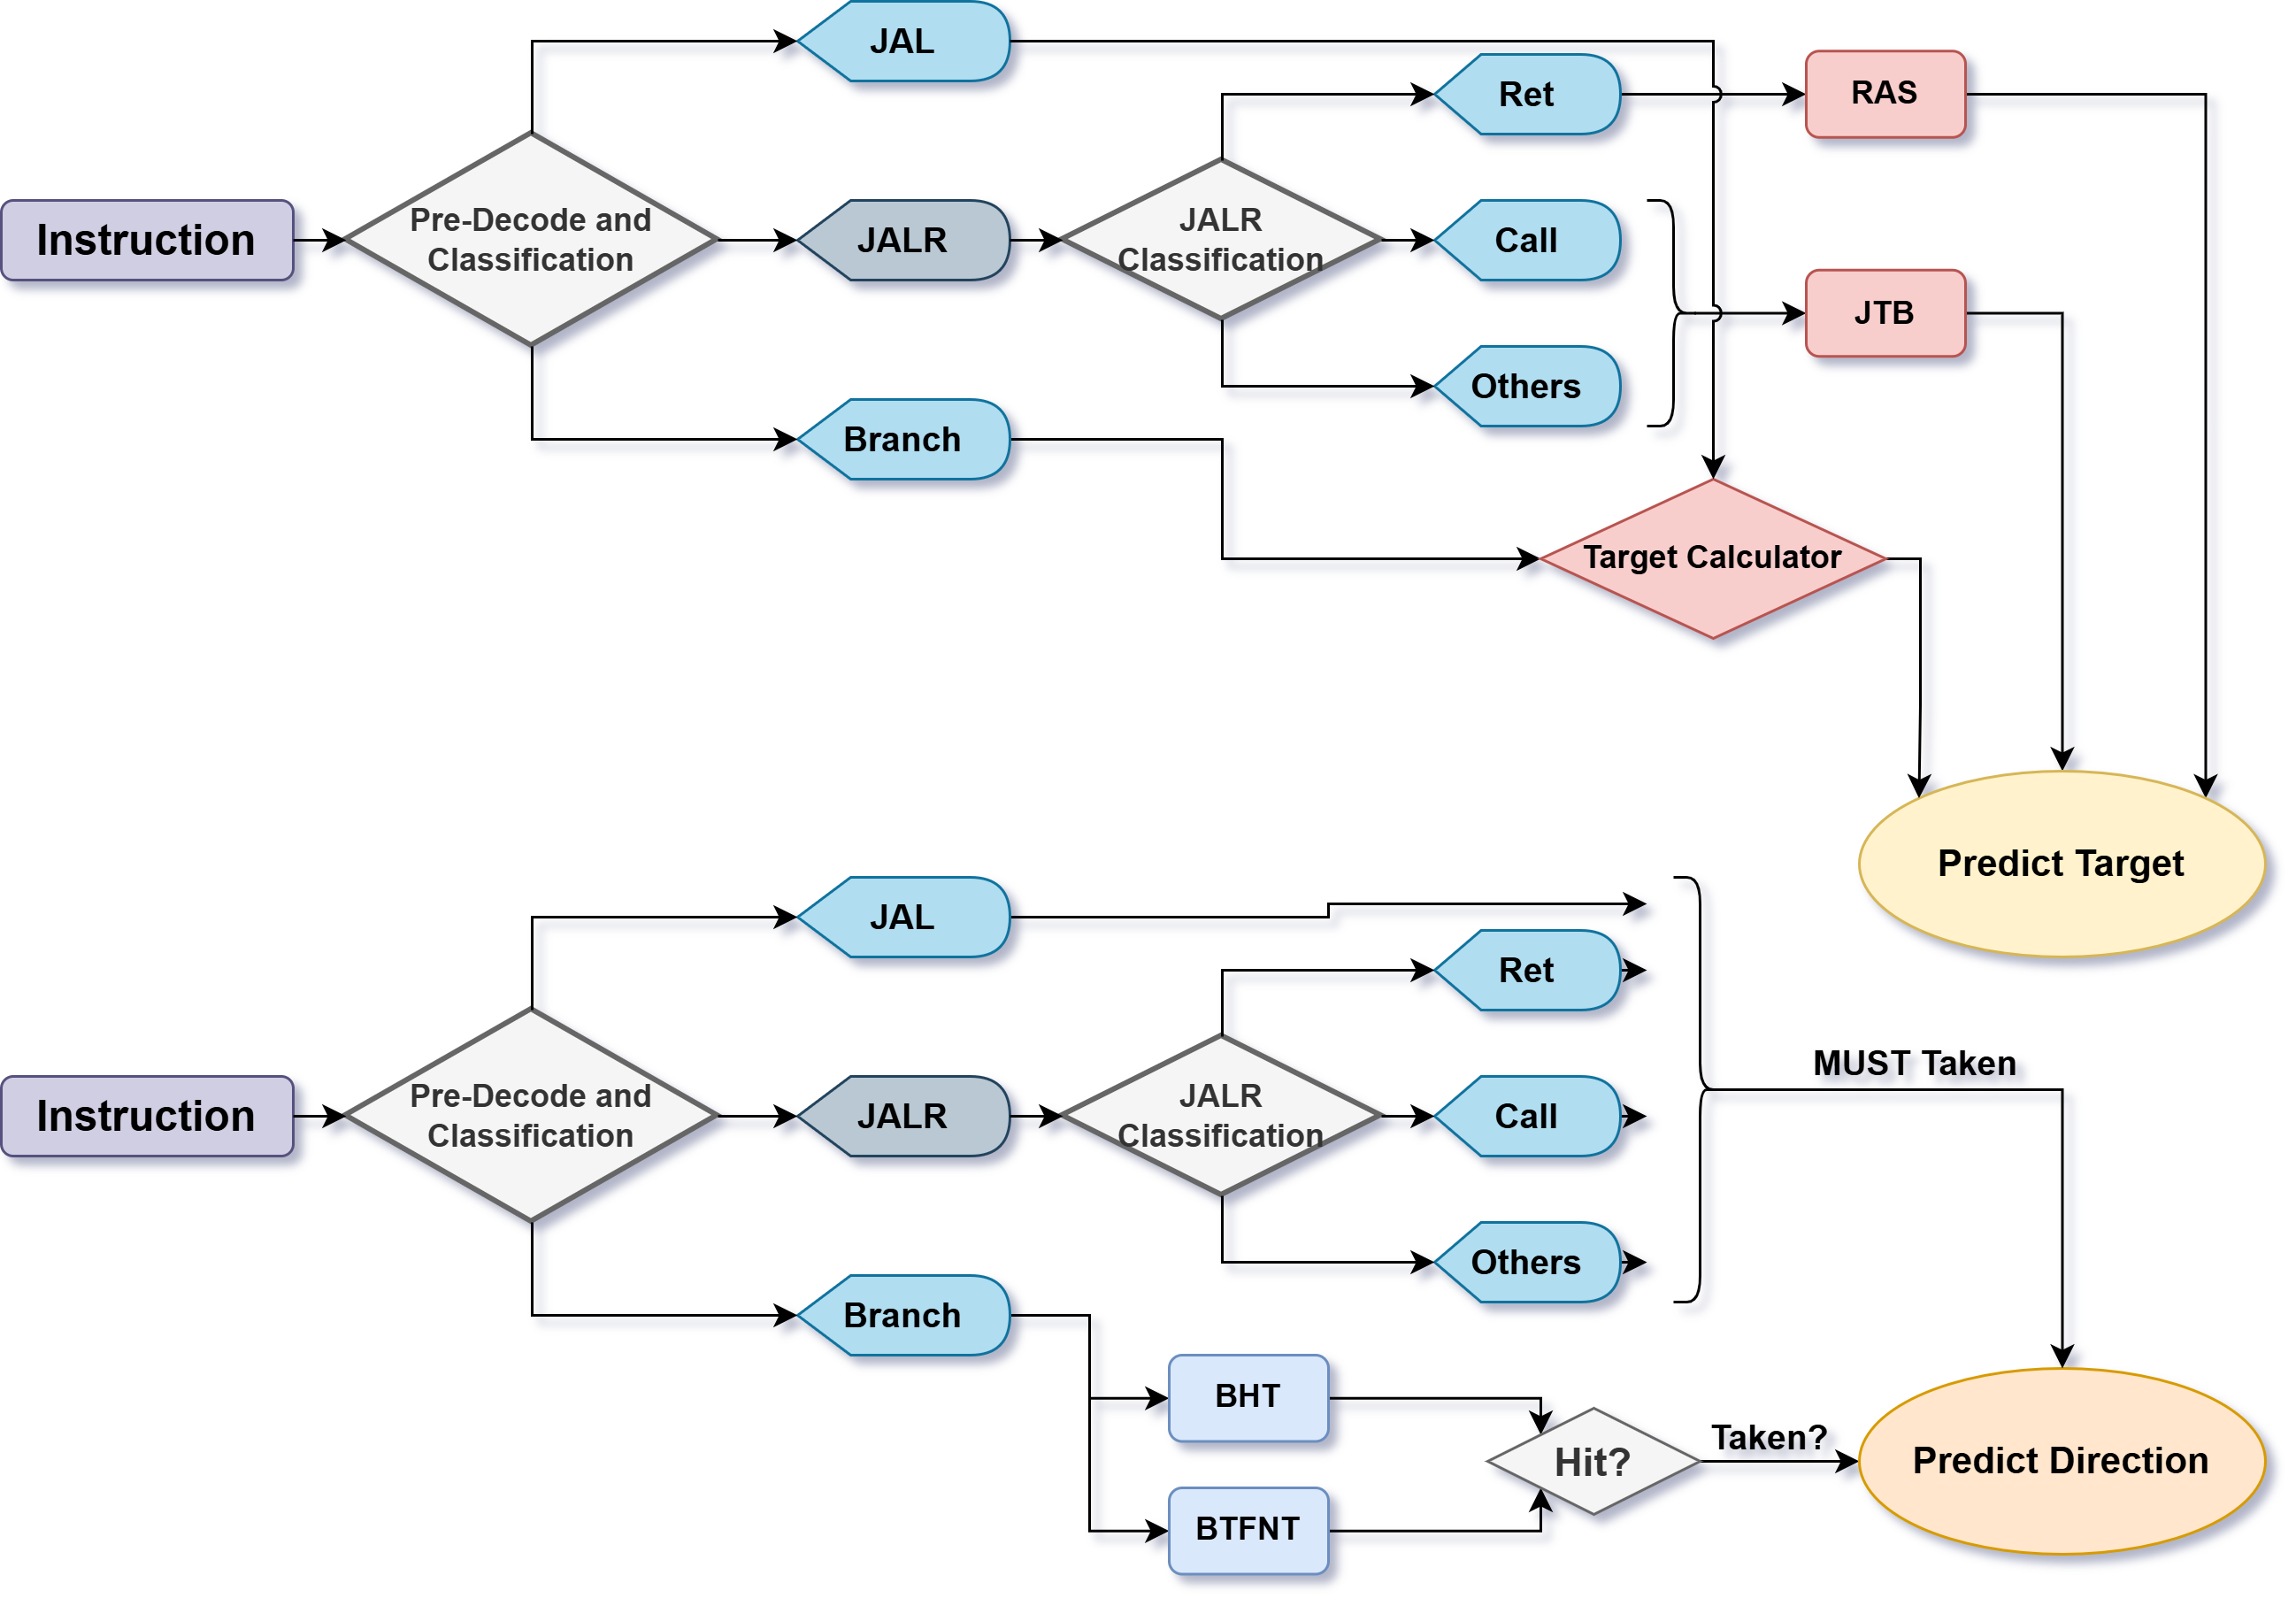
\includegraphics[width=0.8\linewidth]{figures/branch_prediction_summary.png}
        \caption{跳转分支预测模式总结图}
        \label{fig:JBPSummary}
    \end{figure}

    为进一步验证上述分类预测机制的实际效果，本设计以 \texttt{ITERATIONS=1} 的 CoreMark 仿真运行窗口为样本，对不同控制流类型的方向预测与目标预测准确率进行了统计，结果见表~\ref{tab:branch_prediction_accuracy}。该统计不来自 \texttt{ITERATIONS=5000} 的上板 UART 性能输出，而是来自 testbench 在单次迭代仿真中的周期级事件计数。从统计结果可以看出，\texttt{JAL} 与 Branch 的目标地址由于均由 \texttt{PC+IMM} 直接计算，因此目标预测准确率达到 \texttt{100.00\%}；\texttt{JALR} 的目标预测主要由 RAS 与 JTB 提供，仍保持了较高准确率。总体而言，该预测结构在避免大容量 BTB 等复杂结构的前提下，实现了较好的控制流预测效果。
    \begin{table}[H]
        \centering
        \caption{CoreMark 单次迭代仿真跳转分支预测准确率统计}
        \label{tab:branch_prediction_accuracy}
        \begin{tabular}{lcc}
            \toprule
            指令类型 & 方向预测准确率 & 目标预测准确率 \\
            \midrule
            \texttt{JAL} & \texttt{100.00\%} & \texttt{100.00\%} \\
            \texttt{JALR} & \texttt{100.00\%} & \texttt{99.91\%} \\
            Branch & \texttt{87.06\%} & \texttt{100.00\%} \\
            \midrule
            总体 & \multicolumn{2}{c}{\texttt{88.43\%}} \\
            \bottomrule
        \end{tabular}
    \end{table}


\subsection{数据相关阻塞Stall与转发Bypass}
    本设计采用单发射、顺序流动、顺序写回的流水线组织，数据相关主要体现为相邻或近邻指令之间的 RAW（Read After Write）相关。由于不存在乱序执行与乱序写回，WAR 与 WAW 相关不会在当前微架构中形成结构性问题；因此，数据相关处理的核心是：在不破坏顺序语义的前提下，尽量通过转发消除 RAW 等待，并在数据尚未产生时精确阻塞或推迟相关操作。

    对于普通整数运算结果，本设计在 ID 阶段完成源操作数选择，并由 \texttt{forwarding.v} 提供 EX、MEM、WB 三级前递路径。当前译码级读出的 \texttt{rs1}/\texttt{rs2} 数据会按“越新优先”的原则进行选择：若 EX 级、MEM 级、WB 级存在写回使能且写回寄存器号与当前源寄存器号相同，则优先使用对应阶段的待写回数据；否则使用寄存器堆原始读数。其优先级可概括为：
    \[
        EX > MEM > WB > RegFile
    \]
    同时，所有转发判断均排除 \texttt{x0}，以保持 RISC-V 零寄存器语义。该结构可以覆盖普通 ALU 指令之间的大部分相邻 RAW 相关，使后一条指令不必等待前一条指令真正进入 WB 阶段，整体数据转发路径见（图~\ref{fig:dataBypass}）。
    \begin{figure}[H]
        \centering
        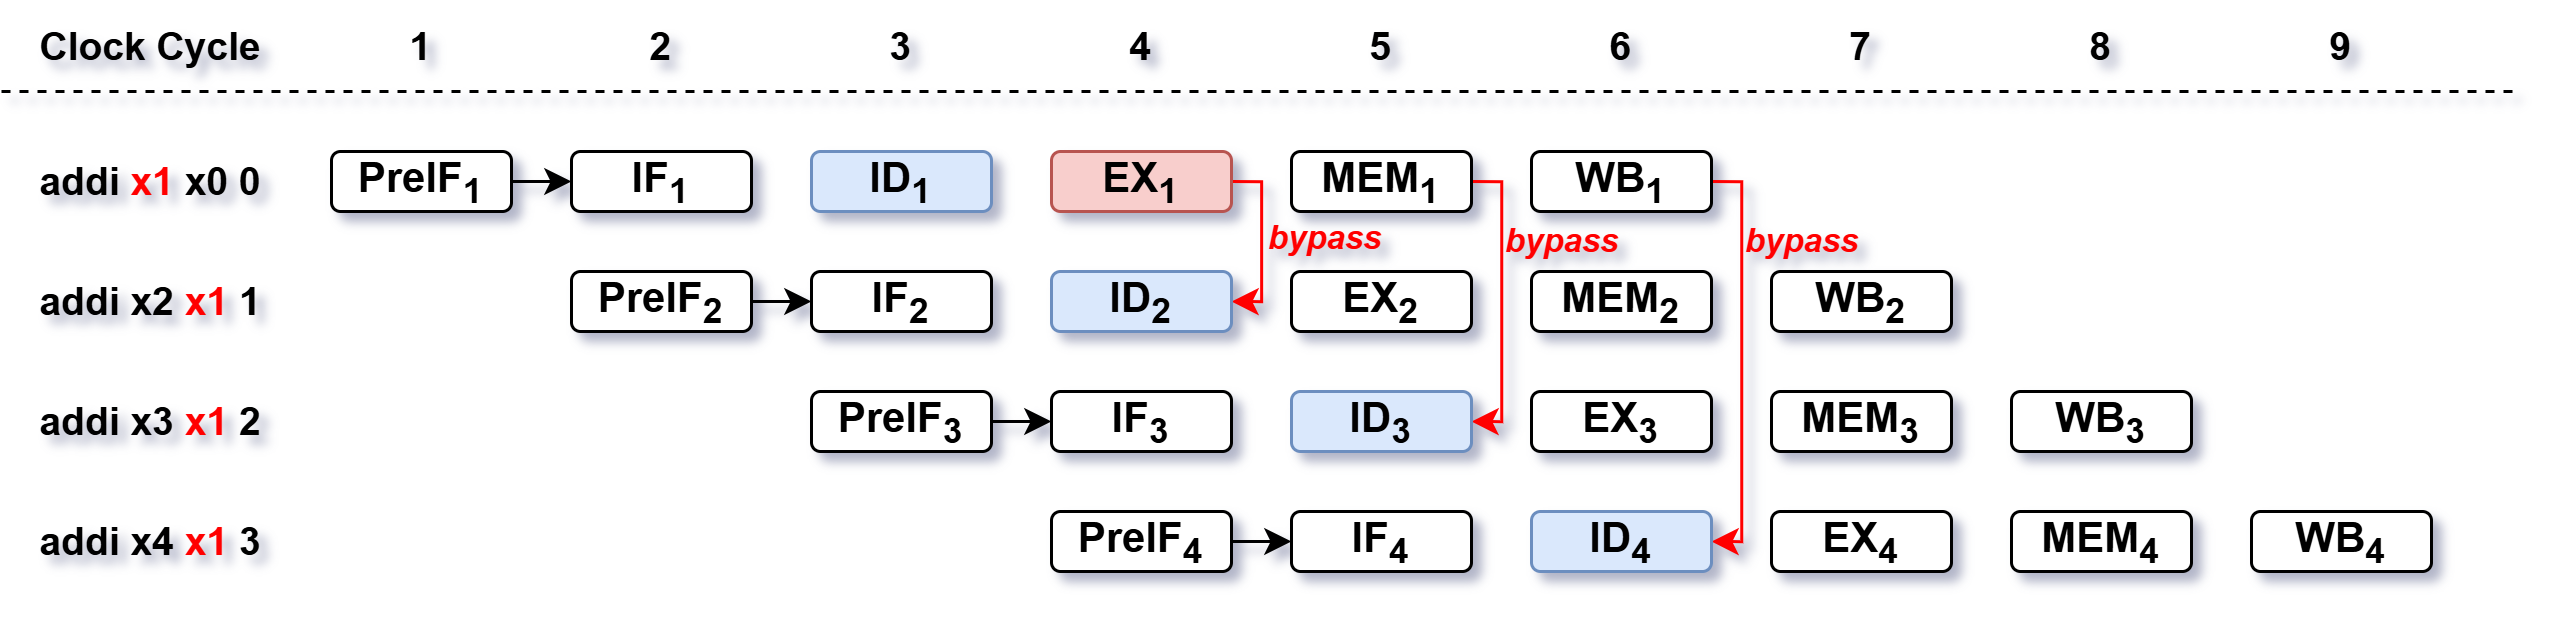
\includegraphics[width=0.85\linewidth]{figures/bypass.png}
        \caption{普通 RAW 数据相关转发路径示意图}
        \label{fig:dataBypass}
    \end{figure}

    对于 \texttt{load-use hazard}，由于 \texttt{LOAD} 指令的数据需要经过存储总线返回，紧随其后的普通指令若立即使用该结果，则 EX 阶段无法在同一拍获得有效操作数。

    此类相关由 \texttt{ctrl\_late\_detect.v} 集中检测。设 EX 级为读存储指令且其目的寄存器有效：
    \[
        load\_rd\_valid = ex\_dmem\_re \land (ex\_rd \ne 0)
    \]
    若 ID 级源寄存器与该目的寄存器相同，则形成 \texttt{rs1}/\texttt{rs2} 的 load-use 匹配：
    \[
        rs1\_match = load\_rd\_valid \land (id\_rs1 = ex\_rd)
    \]
    \[
        rs2\_match = load\_rd\_valid \land (id\_rs2 = ex\_rd)
    \]
    对普通指令而言，只要其实际使用的源寄存器发生上述匹配，即产生普通 load-use hazard。此时流水线通过 \texttt{pipeline\_stall} 阻塞前端与级间寄存器推进一拍，等待 load 数据到达后再由后续转发路径提供正确操作数。阻塞与转发的协同处理关系见（图~\ref{fig:stallAndBypass}）。
    \begin{figure}[H]
        \centering
        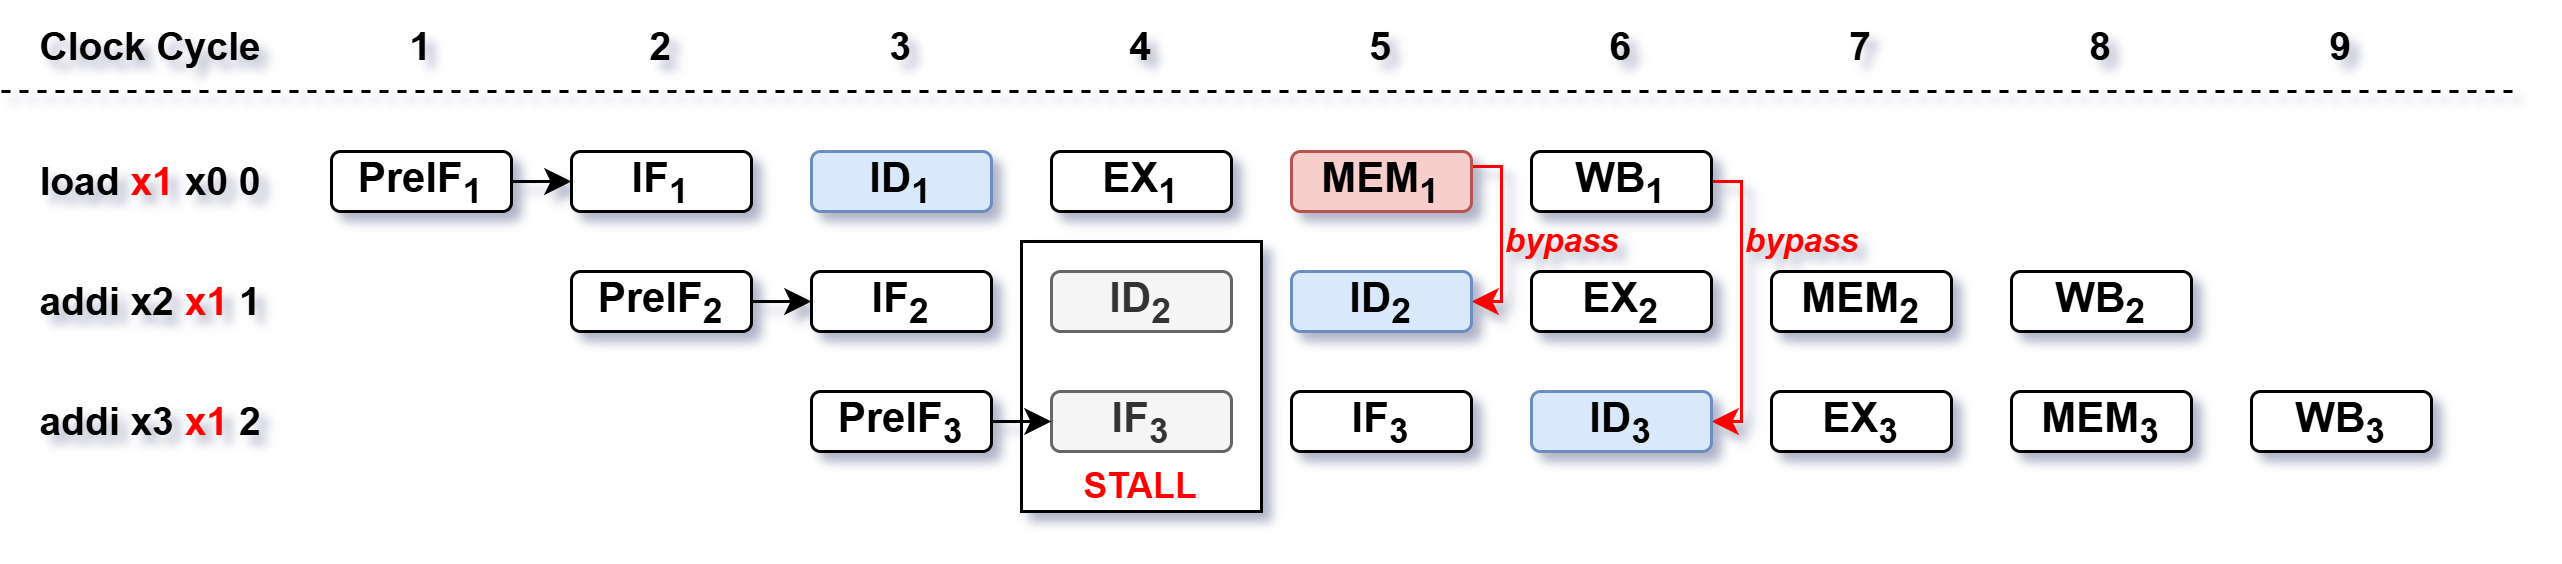
\includegraphics[width=0.9\linewidth]{figures/stall_and_bypass.png}
        \caption{Load-Use 阻塞与数据转发协同处理示意图}
        \label{fig:stallAndBypass}
    \end{figure}

    需要区分的是，乘除法等长延迟运算不使用普通 \texttt{pipeline\_stall} 表示，而是由执行级产生 \texttt{ex\_mul\_busy} 与 \texttt{ex\_div\_busy}，并合成为全局保持信号：
    \[
        pipeline\_hold = ex\_mul\_busy \lor ex\_div\_busy
    \]
    \[
        pipeline\_block = pipeline\_stall \lor pipeline\_hold
    \]
    其中 \texttt{pipeline\_stall} 主要用于短周期 load-use 阻塞，\texttt{pipeline\_hold} 用于保持多周期执行单元占用期间的流水线一致性。这样可以避免将长延迟单元伪装成多次短阻塞，也使阻塞来源在控制逻辑和性能统计上更加清晰。

    对控制类指令，尤其是 Branch 与 \texttt{JALR}，本设计没有简单沿用普通 load-use 阻塞策略，而是引入仅针对 J/B 的晚解析机制。其原因在于，控制类指令依赖 load 结果时，真正需要的是跳转方向或 \texttt{JALR} 目标地址，而不是在 EX 当拍产生普通写回结果。因此，该类相关可以被推迟到 MEM 级结合 load 返回数据解析，从而减少因控制相关造成的停顿周期。

\subsection{针对 J/B 的晚转发方案}
    在普通五级或准六级流水线中，\texttt{load-use hazard} 的标准处理方式是阻塞流水线：当后一条指令需要使用前一条 \texttt{LOAD} 的返回值时，前端和级间寄存器暂停推进，等待数据从存储侧返回后再继续执行。对于普通 ALU 指令、访存地址计算和 store 数据路径，这种处理是必要且直接的，因为这些指令必须在 EX/MEM 阶段得到正确操作数，才能产生后续数据结果或访存行为。

    但是，Branch 与 \texttt{JALR} 依赖 load 结果时，情况并不完全相同。Branch 需要 load 返回值参与条件比较，\texttt{JALR} 需要 load 返回值参与目标地址计算；二者真正受影响的是控制流解析结果，而不是普通寄存器写回数据。更重要的是，这类“load 后紧跟 Branch/\texttt{JALR}”的模式在实际程序中并不罕见，例如循环边界检查、数组遍历、链表/函数指针访问等场景均可能形成此类相关。若仍然沿用标准 load-use 阻塞方案，则不论前端预测最终是否正确，每一条依赖 load 的 J/B 指令都必须先无条件付出 1 拍停顿代价。该方式实现简单，但会把一部分本可后移解析的控制相关也转化为固定前端停顿，增加分支密集程序中的周期损失。

    从代价期望上看，晚转发方案的关键判断在于：它把“所有相关指令都付出 1 拍确定代价”转化为“预测失败的小部分指令付出更晚恢复代价”。若采用晚解析，预测正确时可以避免这 1 拍强制停顿；预测失败时，由于真实控制流在 MEM 级才被确认，需要承担约 3 拍 Flush 恢复代价。考虑到本设计跳转分支预测总体准确率约为 90\%，则只有约 10\% 的依赖 load 的 J/B 指令会落入晚解析失败路径。也就是说，相比于 100\% 的相关 J/B 指令均固定损失 1 拍，晚转发只让约 10\% 的相关 J/B 指令承担更高恢复代价；即使失败场景的单次代价更高，其整体期望损失仍更低，并且预测失败相较普通错误恢复主要体现为解析阶段后移所带来的额外代价。

    因此，本设计的核心思路是：不将所有 load-use 相关都视为同一种数据相关，而是区分“必须立即获得数据的普通数据通路”和“可以后移确认的控制解析通路”。对于普通指令，仍然采用标准阻塞；对于依赖前一条 load 的 Branch 与 \texttt{JALR}，则不立即阻塞，而是将其标记为需要晚解析，使该指令继续向后流动，并在 load 数据已经可用的 MEM 级完成真实控制流解析。标准阻塞方案与 J/B 晚转发方案的流水线代价对比如（图~\ref{fig:lateBypassContrast}）所示。
    \begin{figure}[H]
        \centering
        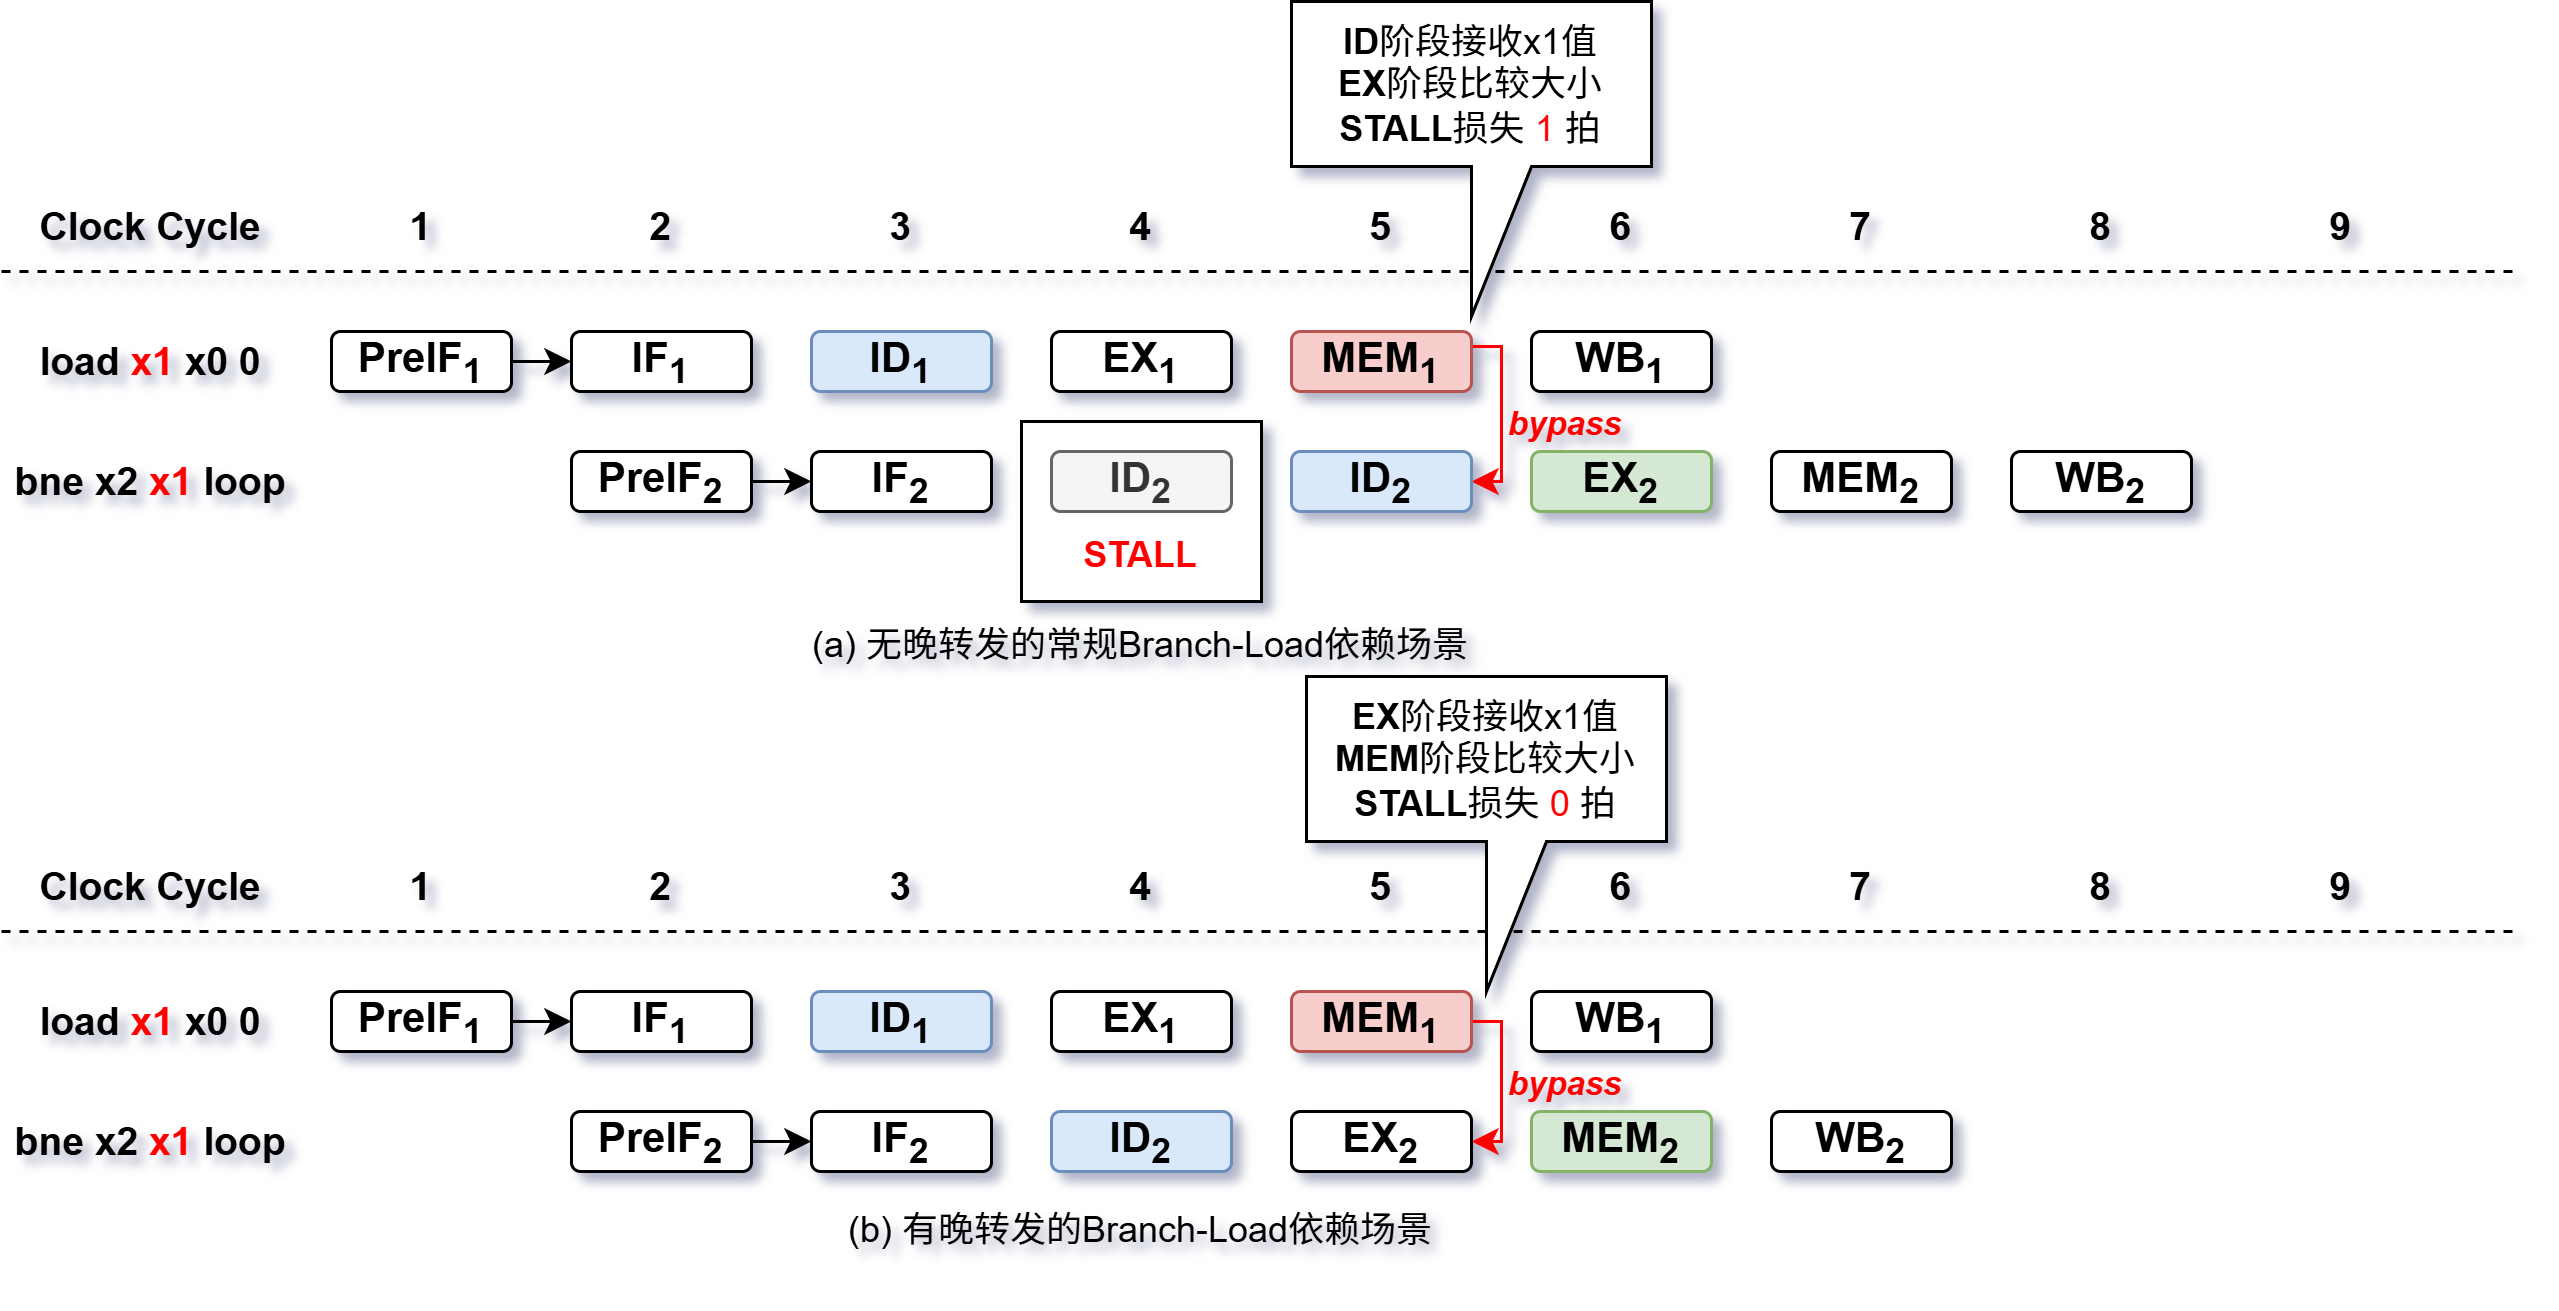
\includegraphics[width=0.95\linewidth]{figures/late_bypass_contrast.png}
        \caption{标准 Load-Use 阻塞与 J/B 晚转发方案对比示意图}
        \label{fig:lateBypassContrast}
    \end{figure}

    为实现这一思路，首先需要解决的问题是如何在 ID 阶段准确区分普通 load-use 与控制类 load-use。对此，\texttt{ctrl\_late\_detect.v} 在检测 EX 级 load 目的寄存器与 ID 级源寄存器匹配的基础上，进一步引入当前指令是否为 Branch 或 \texttt{JALR} 的条件：若普通指令依赖 load，则产生 \texttt{pipeline\_stall}；若 Branch 或 \texttt{JALR} 依赖 load，则置位 \texttt{id\_ctrl\_defer}，将其送入晚解析路径。其检测条件为：
    \[
        id\_ctrl\_dep\_rs1 = (id\_branch \lor id\_jalr) \land rs1\_match
    \]
    \[
        id\_ctrl\_dep\_rs2 = id\_branch \land rs2\_match
    \]
    \[
        id\_ctrl\_defer = id\_ctrl\_dep\_rs1 \lor id\_ctrl\_dep\_rs2
    \]
    因而普通阻塞条件被修正为：
    \[
        pipeline\_stall = normal\_load\_hazard \land \lnot id\_ctrl\_defer
    \]
    这一步完成了第一次划分：普通 ALU、访存地址计算、存储数据等依赖 load 的场景仍会阻塞；只有 Branch 与 \texttt{JALR} 的控制解析被允许后移。

    随后出现的第二个问题是：控制类指令虽然可以后移，但后移后仍必须恢复出完整的真实控制流结果。为此，\texttt{id\_ctrl\_defer}、\texttt{id\_ctrl\_dep\_rs1}、\texttt{id\_ctrl\_dep\_rs2} 等标记随流水线向后传递到 MEM 级，由 \texttt{mem\_ctrl\_resolve.v} 使用 \texttt{wb\_late\_data} 重构真实操作数。对于 Branch，该模块重新执行等于、不等于、有符号小于、无符号小于等比较；对于 \texttt{JALR}，则使用 load 返回值与立即数计算真实目标：
    \[
        target_{jalr} = wb\_late\_data + imm_{jalr}
    \]
    由此，晚解析路径不仅获得了真实跳转方向或目标地址，也保留了与前端预测结果进行一致性检查的能力。若 MEM 级晚解析结果与前端预测结果在方向或目标地址上不一致，则产生 \texttt{mem\_ctrl\_mispredict} 与 \texttt{mem\_ctrl\_redirect\_addr}，触发前端重定向恢复。

    该机制最终只限定在 J/B 指令上，是演进后的边界选择。若将晚解析扩大到普通 ALU 或访存类指令，必须额外处理结果重放、访存撤销、写回顺序和异常边界等问题，控制复杂度会迅速上升；而 Branch 不写回通用寄存器，\texttt{JALR} 的链接地址可由指令 PC 直接确定，其依赖 load 的部分主要影响控制流目标，因此更适合后移到 MEM 级确认。也就是说，本设计不是试图建立通用乱序式重放机制，而是在顺序流水线约束下，选择最能带来收益且代价可控的控制类指令作为优化对象。

    最终，本设计形成了一种仅针对 Branch 与 \texttt{JALR} 的 load-use 晚转发/晚解析机制：ID 级识别控制类 load-use 相关并取消普通停顿，MEM 级利用 load 返回数据完成真实控制流解析与必要重定向。该机制以少量标记位、比较逻辑和 \texttt{JALR} 目标加法为代价，减少了控制类 load-use 场景的无效阻塞，同时避免在 ID/EX 关键路径上叠加额外长组合逻辑，在性能收益、资源开销和时序压力之间取得了较好的折中。

\subsection{乘法器、除法器与长延迟单元}
    本设计支持 \texttt{RV32M} 乘除法扩展，其中乘法与除法均作为执行级长延迟单元接入。ID 阶段识别到乘法或除法类指令后，在不存在冲刷、短阻塞和长保持的条件下产生 \texttt{id\_mul\_preload} 或 \texttt{id\_div\_preload}，将操作数提前送入对应执行单元。这样可以使长延迟单元尽早开始工作，减少由译码到执行之间的额外等待。

    对于 FPGA 平台上的乘法实现，标准方案通常是在指令进入 EX 阶段后再启动 DSP 乘法单元，随后等待 DSP 内部寄存与部分积组合逻辑给出结果。这种方式结构直观，但在单发射顺序流水线中会带来两个问题：其一，DSP 乘法本身具有固定多拍延迟，容易直接转化为 \texttt{pipeline\_hold}；其二，若等到 EX 阶段才装载乘法操作数，则乘法单元启动时机相对滞后，会额外放大长延迟单元对前后级的阻塞影响。因此，本设计没有把乘法器简单视为 EX 阶段内部的纯组合附属逻辑，而是将乘法操作数装载时机前移到 ID 阶段。

    该前移机制的实现关键在于提前识别乘法类 \texttt{ALU} 操作，并在流水线没有冲刷、普通阻塞和长延迟保持时，生成 \texttt{id\_mul\_preload}：
    \[
        id\_mul\_preload = id\_mul\_op \land \lnot pipeline\_flush
                         \land \lnot pipeline\_stall \land \lnot pipeline\_hold
    \]
    同时，译码侧根据具体乘法指令生成 \texttt{id\_mul\_signed\_a} 与 \texttt{id\_mul\_signed\_b}，并将已经完成转发选择后的 \texttt{id\_alu\_num1}、\texttt{id\_alu\_num2} 作为乘法器输入。这样，乘法指令尚未真正成为 EX 级当前指令时，DSP 乘法单元已经开始接收并锁存操作数；当该指令进入 EX 级时，乘法执行进度已经提前推进。该过程本质上是在不改变指令顺序语义的前提下，将长延迟单元的“输入装载阶段”从 EX 前移到 ID，使 DSP 固有延迟尽可能与流水线级间推进重叠。

    该方案的边界也较为明确：只有在流水线未被冲刷、未发生普通 load-use 阻塞、且乘除法单元没有正在保持流水线时，才允许发起 preload。因此，前移不会把错误路径或被阻塞路径的操作数写入乘法器状态，也不会破坏顺序执行下的结果对应关系。最终，本设计通过乘法操作前移机制，在保持 DSP 分块乘法结构和顺序提交模型不变的条件下，压缩了乘法指令启动等待对流水线的影响，为降低 \texttt{mul hold} 周期提供了低资源代价的优化路径。

    \texttt{mul\_unit.v} 采用 FPGA DSP 资源实现 32 位乘法。由于 7 系列 FPGA 的 DSP 乘法输入位宽有限，设计将 32 位操作数拆分为高 16 位与低 16 位，并扩展为 17 位有符号局部操作数，分别计算 \texttt{ll}、\texttt{lh}、\texttt{hl}、\texttt{hh} 四个部分积。四个部分积经移位后重新组合：
    \[
        P = P_{ll} + (P_{lh} \ll 16) + (P_{hl} \ll 16) + (P_{hh} \ll 32)
    \]
    为降低组合加法深度，模块使用平衡加法树完成部分积求和。乘法器固定延迟为 3 拍，综合路径下实例化 \texttt{DSP48E1}，仿真路径下使用行为级乘法模型。通过对操作数符号扩展方式的控制，该单元覆盖 \texttt{MUL}、\texttt{MULH}、\texttt{MULHSU} 与 \texttt{MULHU} 所需的低 32 位和高 32 位结果。

    \texttt{div\_unit.v} 采用迭代式除法结构，以较低面积代价支持 \texttt{DIV}、\texttt{DIVU}、\texttt{REM} 与 \texttt{REMU}。其状态机包括 \texttt{S\_IDLE}、\texttt{S\_PREP}、\texttt{S\_RUN}、\texttt{S\_FIX} 与 \texttt{S\_DONE}。在准备阶段，模块完成除数为零、有符号溢出等特殊情况判断；在运行阶段执行 32 次移位减法迭代；在修正阶段根据有符号运算要求恢复商或余数的符号。对于除零场景，商返回 \texttt{0xffffffff}，余数返回被除数；对于 \texttt{0x80000000 / -1} 的有符号溢出场景，商返回 \texttt{0x80000000}，余数返回 0，符合 RISC-V M 扩展语义。

    当乘法器或除法器尚未给出 \texttt{ready} 时，执行级分别置位 \texttt{ex\_mul\_busy} 或 \texttt{ex\_div\_busy}，并通过 \texttt{pipeline\_hold} 保持流水线。该处理方式保证了多周期单元与顺序流水线之间的状态一致性，但也意味着长延迟指令会直接转化为前后级等待周期。当前乘法虽然已经利用 DSP 与操作数前移降低代价，但固定多拍延迟仍会在乘法密集型 benchmark 中形成明显的 hold 周期；除法则以面积优先为目标，采用迭代结构换取较低资源消耗。后续若继续优化，可考虑进一步流水化乘法结果通路、针对乘法结果增加更细粒度的完成旁路，或在面积允许时引入更高吞吐的除法结构。

\subsection{存储系统与 MMIO}
    本设计采用指令存储器、数据存储器与 MMIO 外设空间相互独立的存储组织，并通过 \texttt{bus\_interconnect.v} 在 CPU 数据访问侧完成地址译码与从设备选择。互连逻辑将 \texttt{IMEM\_BASE\_ADDR} 对应区域映射到指令存储器，将 \texttt{DMEM\_BASE\_ADDR} 对应区域映射到数据存储器，并将高 4 位为 \texttt{0xF} 的地址映射到 MMIO 区域。各区域的具体地址划分已在表~\ref{tab:mem_map} 与表~\ref{tab:mmio_map} 中给出。

    由于 IMEM 与 DMEM 均基于片上 BRAM 实现，其读访问天然具有同步读延迟：地址在当前周期送入存储器后，数据通常需要到下一拍才能稳定返回。若完全按照传统阶段语义处理，即 IF 阶段才向 IMEM 发起访问、MEM 阶段才向 DMEM 发起访问，则取指和访存都会在流水线上暴露出额外等待周期；对于单发射处理器而言，这类等待会直接降低有效 IPC。问题在于，直接改用大规模异步读结构或 Cache 虽然可以隐藏部分延迟，但会带来更高 LUT/BRAM 资源消耗和更复杂的时序路径，不符合本设计低资源实现目标。

    因此，本设计采用访存前移的方式处理 BRAM 固有延迟：对 IMEM，将访问地址前移到 PreIF 阶段给出，使 IF 阶段接收 BRAM 返回的指令；对 DMEM，则在 EX 阶段完成访存地址计算后立即发起数据总线访问，使数据在后续 MEM/WB 路径中可被接收和转发。对于取指路径，\texttt{pc.v} 输出的 \texttt{preif\_pc\_addr} 直接进入 \texttt{imem.v}，IMEM 主读端口在下一拍给出 \texttt{if\_instr\_o}；同时，第二读端口可在动态压缩前端需要时读取 \texttt{PC+4} 候选指令。对于数据路径，执行级计算出的 \texttt{ex\_dmem\_wr\_addr} 直接作为总线地址，顶层由：
    \[
        bus\_m\_stb = (ex\_dmem\_we \lor ex\_dmem\_re) \land \lnot mem\_ctrl\_mispredict
    \]
    发起访问，而不是等到访存指令正式进入 MEM 级后才开始请求存储器。

    这一机制在演进上需要解决两个约束。第一，前移访问不能破坏错误路径恢复，因此数据总线发起条件受 \texttt{mem\_ctrl\_mispredict} 门控，避免更老控制流纠错时错误路径访存继续生效。第二，前移访问仍要保持流水线语义一致，因此 EX/MEM 寄存器继续传递 \texttt{ex\_dmem\_we}、\texttt{ex\_dmem\_re}、访存地址和写数据，MEM/WB 路径再根据返回数据完成写回或晚转发。最终，本设计通过“IMEM 访问前移到 PreIF、DMEM 访问前移到 EX”的方式，在不引入复杂 Cache 的前提下吸收 BRAM 同步读延迟，将原本会显式暴露在 IF/MEM 阶段的等待压缩到流水线自然推进过程中，从而以较低资源代价改善取指与数据访存效率。

    \texttt{imem.v} 使用 \texttt{ram\_style = "block"} 指定片上 BRAM 实现，当前深度为 \texttt{8192} 个 32 位字，即 \texttt{32KiB}。指令内容通过：
    \[
        \texttt{\$readmemh("imem.mem", imem)}
    \]
    在仿真或综合初始化流程中加载。IMEM 的主取指端口为同步读，PreIF 阶段给出 PC 后，IF 阶段获得对应指令；另一读端口在总线读取与前端双取指之间复用，其中总线读取优先。当动态压缩前端需要同时取得下一条候选指令时，该端口可读取 \texttt{PC+4} 对应指令，为前端预测与恢复路径提供支持。

    \texttt{dmem.v} 同样使用 BRAM 实现，但按字节拆分为 4 个 8 位存储体，以支持 \texttt{SB}、\texttt{SH}、\texttt{SW} 的字节使能写入。读路径在时钟边沿锁存 32 位字数据及地址低位，随后根据 \texttt{mem\_op} 完成 \texttt{LB}、\texttt{LH}、\texttt{LW}、\texttt{LBU} 与 \texttt{LHU} 的符号扩展或零扩展。写访问和读访问均通过 \texttt{bus\_ack} 返回完成信号，整体保持一拍同步存储访问模型。

    \texttt{mmio.v} 提供轻量级外设寄存器接口，主要包括 64 位周期计数器低/高 32 位只读寄存器、\texttt{tohost} 程序完成标志、LED 输出寄存器、UART 发送数据寄存器与 UART 状态寄存器。其中 \texttt{UART\_TX} 写入低 8 位后进入发送队列，\texttt{UART\_STATUS} 返回 \texttt{\{overflow,busy,ready\}} 状态；\texttt{INSTRET} 相关地址在当前 RTL 中保留但返回 0。UART 发送由 \texttt{uart\_tx.v} 实现，采用 8N1 串口格式并带 4 项 FIFO；综合默认波特率为 115200，仿真配置下使用更高波特率以缩短输出时间。板级顶层 \texttt{top.v} 还实例化 \texttt{seg7\_display.v}，将 LED 对应的低 16 位值扩展为 32 位后显示在 8 位七段数码管上，便于 FPGA 板上观察运行状态。

    \texttt{imem.mem} 是软件镜像进入硬件系统的直接载体。Benchmark 或裸机程序经 RISC-V 工具链编译、链接和格式转换后，生成按 32 位字排列的十六进制文本文件；仿真与 Vivado 初始化流程均通过该文件填充 IMEM。因此，更换测试程序时不需要修改 RTL，只需重新生成并替换 \texttt{imem.mem}。

\subsection{模块划分说明}
\begin{longtable}{p{0.34\textwidth}p{0.58\textwidth}}
    \caption{主要模块职责} \\
    \toprule
    模块 & 主要职责 \\
    \midrule
    \endfirsthead
    \toprule
    模块 & 主要职责 \\
    \midrule
    \endhead
    \texttt{cpu.v} & CPU 顶层连接，组织前端、译码、执行、访存、写回、总线与外设接口，并完成全局冲刷、阻塞、保持和重定向信号仲裁 \\
    \texttt{top.v} & FPGA 工程顶层封装，例化时钟 IP、CPU、LED/UART 输出与七段数码管显示模块 \\
    \texttt{pc.v} & PC 更新与前端重定向管理，根据预测跳转、错误恢复、阻塞保持等条件选择下一取指地址 \\
    \texttt{frontend\_ctrl.v} & 前端控制整理，完成 IF/slot1 控制流轻量分类、Branch/\texttt{JAL} 目标预计算、RAS/JTB/BHT 结果仲裁，以及动态压缩前端的有效位与冲刷恢复控制 \\
    \texttt{branch\_hash\_mix.v} & BHT 索引哈希生成模块，将 PC 片段与 B 型立即数低位混合，降低小容量 BHT 的别名冲突 \\
    \texttt{branch\_predictor.v} & B 型条件分支方向预测，维护小容量 Tagged BHT 与 2-bit 饱和计数器 \\
    \texttt{jump\_target\_buffer.v} & 非 Ret 类 \texttt{JALR} 目标缓存，保存近期间接跳转目标地址及对应 Tag \\
    \texttt{ras.v} & 返回地址栈，为 Ret 指令提供目标预测，并支持前端双槽位场景下的 shadow 栈顶预测 \\
    \texttt{id.v / ex.v} & 译码与执行级主逻辑，完成指令译码、操作数生成、ALU 运算、跳转解析、访存控制与乘除法单元接入 \\
    \texttt{if\_id.v / id\_ex.v} & 前端到执行前级的流水寄存器，传递指令、PC、预测信息、控制信号与晚解析标记 \\
    \texttt{ex\_mem.v / mem\_wb.v} & 执行到写回阶段的流水寄存器，传递执行结果、访存控制、控制流解析信息与寄存器写回信息 \\
    \texttt{ctrl\_late\_detect.v} & J/B load-use 晚解析检测，区分普通 load-use 阻塞与控制类指令晚转发路径 \\
    \texttt{mem\_ctrl\_resolve.v} & MEM 级控制流晚解析，利用 load 返回数据重新计算 Branch 方向或 \texttt{JALR} 目标，并产生必要重定向 \\
    \texttt{forwarding.v} & ID 阶段源操作数前递选择，按 EX、MEM、WB 优先级解决普通 RAW 相关 \\
    \texttt{regs.v} & 32 个通用寄存器实现，支持双读单写，并保持 \texttt{x0} 恒为 0 \\
    \texttt{pipeline\_stall.v} & 通用 load-use 阻塞检测模块，当前顶层主要由 \texttt{ctrl\_late\_detect.v} 集成等价阻塞逻辑 \\
    \texttt{mul\_unit.v / div\_unit.v} & RV32M 乘除法单元，分别实现 DSP 分块乘法与迭代式除法/取余 \\
    \texttt{bus\_interconnect.v} & 数据访问总线互连，根据地址选择 IMEM、DMEM 或 MMIO 从设备，并返回对应读数据与应答 \\
    \texttt{imem.v / dmem.v} & 指令存储器与数据存储器，均基于片上 BRAM 实现，分别承担程序加载、取指、数据读写与字节/半字扩展 \\
    \texttt{mmio.v} & MMIO 外设寄存器接口，提供周期计数、\texttt{tohost}、LED、UART 发送与 UART 状态访问 \\
    \texttt{uart\_tx.v / seg7\_display.v} & 板级输出辅助模块，分别实现串口发送队列与七段数码管动态显示 \\
    \bottomrule
\end{longtable}

\section{Verilog / VHDL 建模规范}

\subsection{总体原则}
\begin{itemize}
    \item 功能分属明确，避免大段裸露逻辑堆叠在顶层；
    \item 参数尽量集中管理，如统一收敛到 \texttt{defines.v}；
    \item 组合逻辑与时序逻辑边界清晰；
    \item 模块接口职责单一、命名统一；
    \item 优先从根因解决问题，避免补丁式堆叠修改。
\end{itemize}

\subsection{命名规范}
本工程 RTL 以 Verilog 为主，命名遵循“按流水级归属前缀、按信号功能后缀”的原则，尽量使信号含义可以从名称中直接判断。
\begin{itemize}
    \item 模块名与文件名保持一致，采用小写下划线形式，例如 \texttt{branch\_predictor.v}、\texttt{mem\_ctrl\_resolve.v}。
    \item 流水级相关信号使用 \texttt{preif\_}、\texttt{if\_}、\texttt{id\_}、\texttt{ex\_}、\texttt{mem\_}、\texttt{wb\_} 前缀区分所属阶段。
    \item 控制信号按用途使用统一后缀，如 \texttt{\_valid}、\texttt{\_we}、\texttt{\_re}、\texttt{\_stall}、\texttt{\_flush}、\texttt{\_hold}。
    \item 地址、数据与寄存器编号分别使用 \texttt{\_addr}、\texttt{\_data}、\texttt{\_w\_addr} 等后缀，避免混淆数据值与索引值。
    \item 全局参数和宏定义集中放在 \texttt{defines.v} 中，采用大写命名，如 \texttt{IMEM\_BASE\_ADDR}、\texttt{BR\_PRED\_INDEX\_BITS}。
\end{itemize}

\subsection{时序逻辑规范}
时序逻辑统一以系统主时钟 \texttt{clk} 驱动，复位信号为 \texttt{rst\_n}，复位有效性与工程宏定义保持一致。所有寄存器更新均放在 \texttt{always @(posedge clk)} 中，并使用非阻塞赋值。
\begin{itemize}
    \item 级间寄存器负责保存跨阶段信号，避免组合逻辑跨越过多流水级。
    \item 冲刷、阻塞和保持信号在级间寄存器中统一处理，优先级应明确，不在多个模块中重复仲裁。
    \item 多周期单元通过 \texttt{busy}/\texttt{ready} 与流水线保持逻辑交互，避免隐式等待。
    \item 预测器、RAS、JTB 等状态结构只在确认路径或受控更新条件下写入，避免错误路径污染状态。
\end{itemize}

\subsection{组合逻辑规范}
组合逻辑主要用于译码、数据选择、地址计算、预测仲裁和简单比较。简单布尔表达式优先使用 \texttt{assign}，多分支选择或复杂条件判断使用 \texttt{always @*}。
\begin{itemize}
    \item \texttt{always @*} 中必须给输出或中间变量提供默认值，避免综合出锁存器。
    \item 组合路径应避免同时包含大规模比较、加法、查表和多级选择；必要时通过流水级拆分。
    \item 关键路径上的选择逻辑应尽量保持单一职责，例如前端预测仲裁、MEM 级晚解析和写回数据选择分别处理。
    \item 对状态表查找结果应显式给出命中条件，例如 \texttt{valid} 与 \texttt{tag} 同时匹配后才认为预测有效。
\end{itemize}

\subsection{模块化规范}
\texttt{cpu.v} 作为顶层连接模块，只保留必要的数据通路连接与全局选择逻辑；复杂功能应拆分到独立模块中实现。
\begin{itemize}
    \item 前端预测相关逻辑拆分为 BHT、JTB、RAS、哈希混合与前端控制模块，便于单独修改和验证。
    \item 流水线控制类逻辑独立封装，例如 \texttt{ctrl\_late\_detect.v} 负责晚解析检测，\texttt{mem\_ctrl\_resolve.v} 负责 MEM 级控制流恢复。
    \item 存储与外设通过总线互连隔离，IMEM、DMEM、MMIO、UART 等模块职责清晰。
    \item 乘除法单元独立于普通 ALU 主路径，减少执行级主逻辑复杂度。
\end{itemize}

\subsection{参数化规范}
可调整规模的结构均通过 \texttt{defines.v} 统一参数化，避免在多个 RTL 文件中散落常量。
\begin{itemize}
    \item 存储容量由 \texttt{IMEM\_WORD\_ADDR\_BITS}、\texttt{DMEM\_WORD\_ADDR\_BITS} 等参数控制。
    \item 分支预测器规模由 \texttt{BR\_PRED\_INDEX\_BITS}、\texttt{BR\_PRED\_TAG\_BITS}、\texttt{RAS\_DEPTH} 等参数控制。
    \item MMIO 地址、UART 波特率、CPU 时钟频率等平台相关配置集中定义，便于仿真和综合环境切换。
    \item 修改参数后应同步检查位宽截断、索引范围和地址范围，避免出现隐式溢出。
\end{itemize}

\section{验证计划与测试报告}

\subsection{验证目标}
本章基于当前工程保存的验证报告与原始输出，对 \texttt{SXQ-RV32IM CPU} 的功能正确性、benchmark 运行结果、跳转分支预测统计以及 FPGA 实现结果进行汇总。验证目标主要包括：
\begin{enumerate}
    \item 验证目标 \texttt{RV32IM} 裸机指令子集的功能正确性；
    \item 验证前端压缩、预测、阻塞、转发、乘除法与访存路径等关键微架构机制；
    \item 通过 CoreMark、Dhrystone 与 Embench-WikiSort 验证真实程序执行稳定性；
    \item 结合 Vivado 实现报告确认资源、时序、功耗与热稳定性满足当前设计目标。
\end{enumerate}

\subsection{验证环境与数据来源}
当前 CPU 面向 \texttt{RV32IM} 裸机 benchmark 场景，目标工作频率为 \texttt{100 MHz}，FPGA 器件为 \texttt{xc7a100tcsg324-1}。Benchmark 编译工具链统一为 \texttt{riscv64-unknown-elf-gcc}，主测试配置采用 \texttt{-march=rv32im -mabi=ilp32 -mstrict-align -O2}。报告数据来源见表~\ref{tab:validation_sources}，测试环境与构建配置见表~\ref{tab:validation_env}。

\begin{table}[H]
    \centering
    \caption{验证数据来源}
    \label{tab:validation_sources}
    \begin{tabularx}{\textwidth}{lX}
        \toprule
        数据类别 & 来源文件或报告 \\
        \midrule
        Benchmark 原始输出 & 上板运行实际 UART 输出，其中 CoreMark Score 使用 \texttt{ITERATIONS=5000} \\
        跳转分支预测准确率、IPC 等性能指标 & Vivado 仿真输出，其中 CoreMark 周期数、退役指令数、IPC 与预测统计使用 \texttt{ITERATIONS=1} \\
        FPGA 资源占用 & \texttt{top\_utilization\_placed.rpt} \\
        FPGA 时序结果 & \texttt{top\_timing\_summary\_postroute\_physopted.rpt} \\
        FPGA 功耗结果 & \texttt{top\_power\_routed.rpt} \\
        布线状态与 DRC & \texttt{top\_route\_status.rpt}、\texttt{top\_drc\_routed.rpt} \\
        \bottomrule
    \end{tabularx}
\end{table}

\begin{table}[H]
    \centering
    \caption{测试环境与构建配置}
    \label{tab:validation_env}
    \begin{tabularx}{\textwidth}{lX}
        \toprule
        项目 & 配置 \\
        \midrule
        FPGA 器件 & \texttt{xc7a100tcsg324-1} \\
        目标频率 & \texttt{100 MHz} \\
        工具链 & \texttt{riscv64-unknown-elf-gcc} \\
        testbench & \texttt{sim\_1/new/cpu\_tb.v} \\
        指令测试 & \texttt{sources\_1/new/RISCV-TEST} \\
        CoreMark & Score 上板运行使用 \texttt{-march=rv32im -mabi=ilp32 -mstrict-align -O2}，\texttt{ITERATIONS=5000}；周期数、退役指令数、IPC 与预测统计仿真使用同一编译配置下的 \texttt{ITERATIONS=1} \\
        Dhrystone & \texttt{-march=rv32im -mabi=ilp32 -mstrict-align -O2 -std=gnu89}，\texttt{1800 runs}，\texttt{DHRY\_HZ=100000000} \\
        Embench-WikiSort & \texttt{-march=rv32im -mabi=ilp32 -mstrict-align -O2 -std=gnu11}，\texttt{GLOBAL\_SCALE\_FACTOR=1}，\texttt{WARMUP\_HEAT=1} \\
        \bottomrule
    \end{tabularx}
\end{table}

\subsection{功能覆盖与测试内容}
当前设计目标为裸机 \texttt{RV32IM} 计算子集，覆盖基础整数计算、访存、控制转移和 M 扩展乘除法指令。系统级机制如特权级、CSR、异常/中断、虚拟内存、\texttt{FENCE/FENCE.I} 等不作为当前有效功能路径。基于当前目标 ISA，指令类别覆盖情况如表~\ref{tab:validation_isa_coverage} 所示。

\begin{table}[H]
    \centering
    \caption{目标 \texttt{RV32IM} 指令覆盖率}
    \label{tab:validation_isa_coverage}
    \begin{tabularx}{\textwidth}{lcccX}
        \toprule
        指令类别 & 目标指令数 & 已覆盖指令数 & 覆盖率 & 覆盖内容 \\
        \midrule
        U 型立即数 & 2 & 2 & \texttt{100\%} & \texttt{LUI, AUIPC} \\
        整数运算 & 19 & 19 & \texttt{100\%} & R 型与 I 型整数算术、逻辑、移位、比较指令 \\
        控制转移 & 8 & 8 & \texttt{100\%} & \texttt{JAL, JALR} 与六类 B 型条件分支 \\
        Load/Store & 8 & 8 & \texttt{100\%} & 字节、半字、字粒度加载与存储 \\
        M 扩展 & 8 & 8 & \texttt{100\%} & \texttt{MUL/MULH/MULHSU/MULHU/DIV/DIVU/REM/REMU} \\
        \midrule
        合计 & 45 & 45 & \texttt{100\%} & 当前裸机 \texttt{RV32IM} 目标功能全集 \\
        \bottomrule
    \end{tabularx}
\end{table}

工程中的 \texttt{riscv-tests} 适配目录提供 \texttt{38} 个 \texttt{RV32I} 测试程序和 \texttt{8} 个 \texttt{RV32M} 测试程序，合计 \texttt{46} 个官方测试入口，用于覆盖单指令功能、访存、分支跳转以及乘除法行为。主要测试项分解见表~\ref{tab:validation_items}。

\begin{table}[H]
    \centering
    \caption{测试内容分解}
    \label{tab:validation_items}
    \begin{tabularx}{\textwidth}{l l l X}
        \toprule
        测试类别 & 目的 & 状态 & 备注 \\
        \midrule
        RV32I 基础指令 & 验证基础整数功能 & 已完成 & 覆盖整数运算、访存和控制转移路径 \\
        RV32M 扩展指令 & 验证乘除法功能 & 已完成 & 覆盖乘法、除法和取余指令 \\
        分支与跳转 & 验证 \texttt{B/J/JALR} 路径 & 已完成 & CoreMark 单次迭代仿真窗口内进行方向与目标预测统计 \\
        数据相关 & 验证转发与阻塞 & 已完成 & 覆盖普通 RAW、load-use、乘除法 hold 与 J/B 晚解析路径 \\
        前端机制 & 验证前端压缩与预测协同 & 已完成 & 覆盖 PreIF/IF 取指、双槽位前瞻和重定向恢复 \\
        Benchmark & 验证程序级性能 & 已完成 & CoreMark、Dhrystone 与 Embench-WikiSort 均完成有效性校验 \\
        \bottomrule
    \end{tabularx}
\end{table}

\subsection{Benchmark 性能验证}
Benchmark 汇总结果如表~\ref{tab:validation_benchmark_summary} 所示。需要严格区分的是，CoreMark 的 Score 与微架构统计指标不是同一次采集得到：\texttt{275.921925 Iter/s} 来自 \texttt{ITERATIONS=5000} 的实际上板 UART 输出；CoreMark 的周期数 \texttt{C}、退役指令数 \texttt{I}、IPC 以及跳转分支预测准确率来自 \texttt{ITERATIONS=1} 的 Vivado 仿真统计。这样处理是因为 CoreMark 官方性能成绩需要足够长的上板运行时间保证有效性，而周期级退役统计和预测器事件统计若在仿真中运行 \texttt{5000} 次迭代会显著增加验证时间；单次迭代仿真仍覆盖 CoreMark 的主要程序路径，可用于表征当前微架构的周期、退役和控制流行为。IPC 统计采用 testbench 中有效运行窗口内的后端退役口径，即统计周期数 \texttt{C} 与退役指令数 \texttt{I}，并计算：
\[
    \mathrm{IPC}=\frac{I}{C}.
\]

\begin{table}[H]
    \centering
    \caption{Benchmark 汇总结果}
    \label{tab:validation_benchmark_summary}
    \begin{tabularx}{\textwidth}{lccccX}
        \toprule
        Benchmark & Score & IPC & 周期数 C & 退役指令数 I & 有效性说明 \\
        \midrule
        CoreMark & \texttt{275.921925 Iter/s} & \texttt{0.851} & \texttt{362458} & \texttt{308288} & Score 为上板 \texttt{5000} 次迭代结果；C/I/IPC 为 \texttt{1} 次迭代仿真统计 \\
        Dhrystone & \texttt{166000 Dhrystones/s} & \texttt{0.907} & \texttt{1081810} & \texttt{980993} & 输出变量与参考值一致 \\
        Embench-WikiSort & \texttt{122.58} & \texttt{0.786} & \texttt{2965138} & \texttt{2330989} & \texttt{WS V=1}，校验通过 \\
        \bottomrule
    \end{tabularx}
\end{table}

其中，CoreMark Score 使用 \texttt{5000} 次上板迭代，运行时间为 \texttt{18.121068 s}，达到 \texttt{275.921925 Iter/s}，折合 \texttt{2.759219 CoreMark/MHz}；表中的 CoreMark IPC、周期数和退役指令数则来自 \texttt{1} 次迭代仿真，不用于反推 \texttt{5000} 次上板运行时间。Dhrystone 达到 \texttt{166000 Dhrystones/s}，按 \(\mathrm{DMIPS/MHz}=\mathrm{Dhrystones/s}/(1757\times f_{\mathrm{MHz}})\) 计算为 \texttt{0.945 DMIPS/MHz}；Embench-WikiSort 输出 \texttt{WS V=1 S=122.58}，说明排序 benchmark 结果校验通过。

\subsection{跳转分支预测统计}
分支/跳转预测统计来自 \texttt{ITERATIONS=1} 的 CoreMark Vivado 仿真窗口，而不是 \texttt{ITERATIONS=5000} 的上板 UART 性能输出。采用该口径是为了在合理仿真时间内获得周期级控制流事件统计。方向准确率表示控制流方向预测正确比例；目标准确率表示预测 taken 或跳转目标时目标地址正确比例；总体准确率为综合方向与目标后的控制流预测正确比例。统计结果见表~\ref{tab:validation_branch_stats}。

\begin{table}[H]
    \centering
    \caption{CoreMark 单次迭代仿真分支与跳转预测统计}
    \label{tab:validation_branch_stats}
    \begin{tabular}{lcccc}
        \toprule
        类型 & 执行次数 & 方向准确率 & 目标准确率 & 总体准确率 \\
        \midrule
        B 型条件分支 & \texttt{62294} & \texttt{87.06\%} & \texttt{100.00\%} & \texttt{87.06\%} \\
        JAL & \texttt{5230} & \texttt{100.00\%} & \texttt{100.00\%} & \texttt{100.00\%} \\
        JALR & \texttt{2136} & \texttt{100.00\%} & \texttt{99.91\%} & \texttt{99.91\%} \\
        \midrule
        全部控制流指令 & \texttt{69660} & \texttt{88.43\%} & \texttt{99.99\%} & \texttt{88.43\%} \\
        \bottomrule
    \end{tabular}
\end{table}

总体 miss rate 为 \texttt{11.57\%}。由于 \texttt{JAL} 和 \texttt{JALR} 在当前程序中预测准确率很高，主要预测损失来自 B 型条件分支方向预测错误。

\subsection{FPGA 实现验证}
当前版本在 \texttt{xc7a100tcsg324-1} 上完成 placed/post-route 实现，Vivado 报告显示资源占用、时序和功耗均满足当前设计目标。关键实现结果见表~\ref{tab:validation_impl_summary}。

\begin{table}[H]
    \centering
    \caption{FPGA 实现结果汇总}
    \label{tab:validation_impl_summary}
    \begin{tabularx}{\textwidth}{lX}
        \toprule
        指标 & 结果 \\
        \midrule
        Slice LUTs & \texttt{3581}（\texttt{5.65\%}） \\
        Slice Registers & \texttt{2741}（\texttt{2.16\%}） \\
        Block RAM Tile & \texttt{16}（\texttt{11.85\%}） \\
        DSP & \texttt{4}（\texttt{1.67\%}） \\
        WNS / TNS & \texttt{0.050 ns / 0.000 ns} \\
        WHS / THS & \texttt{0.142 ns / 0.000 ns} \\
        约束状态 & \texttt{All user specified timing constraints are met} \\
        总片上功耗 & \texttt{0.329 W} \\
        动态功耗 / 静态功耗 & \texttt{0.231 W / 0.099 W} \\
        结温 & \texttt{26.5}$\,^{\circ}\mathrm{C}$ \\
        \bottomrule
    \end{tabularx}
\end{table}

\subsection{验证结论}
当前版本已完成目标 \texttt{RV32IM} 指令子集、官方 \texttt{riscv-tests} 入口、三类 benchmark 以及 FPGA post-route 实现结果的验证闭环。Benchmark 方面，CoreMark 上板 \texttt{5000} 次迭代运行达到 \texttt{275.921925 Iter/s}，Dhrystone 达到 \texttt{166000 Dhrystones/s}，Embench-WikiSort 得分为 \texttt{122.58}；微架构统计方面，CoreMark 单次迭代仿真窗口内 IPC 为 \texttt{0.851}，总体控制流预测准确率为 \texttt{88.43\%}；FPGA 实现方面，当前设计占用 \texttt{3581} 个 LUT、\texttt{2741} 个 FF、\texttt{16} 个 BRAM Tile 和 \texttt{4} 个 DSP，并在 \texttt{100 MHz} 下满足 post-route 时序约束。综合来看，当前验证结果能够支撑本文关于低资源、低功耗与较高单发射性能的设计结论。

\section{FPGA 适配指南}

\subsection{平台信息}
本设计面向 Digilent Nexys A7-100T 开发板及其对应的 Artix-7 FPGA 器件完成适配。工程顶层由 \texttt{top.v} 负责连接 CPU、时钟 IP、MMIO 外设、UART、LED 和数码管等板级接口，CPU 内部通过片上 BRAM 实现指令存储器与数据存储器，并通过 MMIO 地址空间访问板级外设。平台基础信息如表~\ref{tab:fpga_platform_info} 所示。

\begin{table}[H]
    \centering
    \caption{FPGA 平台信息}
    \label{tab:fpga_platform_info}
    \begin{tabularx}{\textwidth}{lX}
        \toprule
        项目 & 内容 \\
        \midrule
        FPGA 器件 & \texttt{xc7a100tcsg324-1} \\
        开发板 & \texttt{Nexys A7-100T} \\
        约束文件 & \texttt{constrs\_1/new/Artix7T100.xdc} \\
        顶层模块 & \texttt{sources\_1/new/top.v} \\
        CPU 顶层 & \texttt{sources\_1/new/cpu.v} \\
        主时钟 & \texttt{100 MHz}，由 \texttt{clk\_main\_100mhz} 时钟 IP 生成 \\
        板级输出 & UART、LED、七段数码管 \\
        \bottomrule
    \end{tabularx}
\end{table}

\subsection{工程组织与镜像加载}
工程源码主要位于 \texttt{sources\_1/new} 目录。CPU 相关 RTL 包括流水线顶层、前端控制、预测器、译码执行、阻塞转发、乘除法单元、存储器与 MMIO 等模块；约束文件位于 \texttt{constrs\_1/new}；仿真 testbench 位于 \texttt{sim\_1/new}。主要文件组织如表~\ref{tab:fpga_file_layout} 所示。

\begin{table}[H]
    \centering
    \caption{FPGA 工程文件组织}
    \label{tab:fpga_file_layout}
    \begin{tabularx}{\textwidth}{lX}
        \toprule
        路径或文件 & 作用 \\
        \midrule
        \texttt{sources\_1/new/top.v} & FPGA 工程顶层，连接 CPU、时钟、UART、LED、数码管等板级接口 \\
        \texttt{sources\_1/new/cpu.v} & CPU 顶层，连接流水级、预测器、存储器、MMIO 与控制路径 \\
        \texttt{sources\_1/new/defines.v} & 全局参数、地址空间、预测器规模和控制宏定义 \\
        \texttt{sources\_1/new/imem.v}、\texttt{sources\_1/new/dmem.v} & 片上指令/数据存储器，基于 BRAM 组织 \\
        \texttt{sources\_1/new/imem.mem} & 指令镜像初始化文件，由 benchmark 或指令测试程序生成 \\
        \texttt{sources\_1/new/mmio.v} & MMIO 外设接口，连接周期计数、tohost、LED 与 UART 发送路径 \\
        \texttt{sim\_1/new/cpu\_tb.v} & 仿真验证 testbench，用于 benchmark 运行窗口、IPC 与预测统计 \\
        \texttt{constrs\_1/new/Artix7T100.xdc} & Nexys A7-100T 管脚与时钟约束 \\
        \bottomrule
    \end{tabularx}
\end{table}

程序运行前需要将目标测试程序或 benchmark 编译为 \texttt{imem.mem}，并放置在 \texttt{sources\_1/new} 目录下。综合和仿真时，IMEM 通过该文件初始化指令内容；DMEM 则用于运行时数据读写。当前 MMIO 地址空间用于输出运行状态、UART 结果和 benchmark 结束标志，便于在仿真和上板环境中复用同一套软件输出路径。

\subsection{资源与时序结果}
当前版本已完成 Vivado placed/post-route 实现，并在 \texttt{100 MHz} 目标频率下满足所有用户指定时序约束。综合与实现结果如表~\ref{tab:fpga_impl_result} 所示。

\begin{table}[H]
    \centering
    \caption{综合与实现结果}
    \label{tab:fpga_impl_result}
    \begin{tabularx}{\textwidth}{lX}
        \toprule
        项目 & 结果 \\
        \midrule
        LUT / FF / BRAM / DSP & \texttt{3581 / 2741 / 16 / 4} \\
        LUT 占用率 & \texttt{5.65\%} \\
        WNS / TNS & \texttt{0.050 ns / 0.000 ns} \\
        WHS / THS & \texttt{0.142 ns / 0.000 ns} \\
        布线状态 & \texttt{5798 / 5798} 条 routable nets 完成布线，routing errors 为 \texttt{0} \\
        状态 & \texttt{All user specified timing constraints are met} \\
        \bottomrule
    \end{tabularx}
\end{table}

资源消耗主要来自流水线控制、译码、旁路、分支预测、总线互连与 MMIO 控制逻辑；BRAM 主要用于 IMEM 与 DMEM；DSP 主要用于乘法相关数据路径。功耗方面，Vivado post-route 报告显示总片上功耗为 \texttt{0.329 W}，其中动态功耗为 \texttt{0.231 W}，静态功耗为 \texttt{0.099 W}，结温为 \texttt{26.5}$\,^{\circ}\mathrm{C}$，具有较大的热稳定裕量。

\subsection{编译与下载流程}
FPGA 适配流程主要包括软件镜像生成、工程检查、综合实现和上板运行四个阶段。基本流程如下：
\begin{enumerate}
    \item 使用 RISC-V 交叉编译工具链生成目标程序，并转换得到 \texttt{imem.mem}；
    \item 将 \texttt{imem.mem} 放入 \texttt{sources\_1/new}，确认 Vivado 工程引用的是当前镜像文件；
    \item 检查 RTL 源文件、时钟 IP、约束文件和顶层模块连接关系，确认目标器件为 \texttt{xc7a100tcsg324-1}；
    \item 运行 Synthesis，检查是否存在语法错误、未连接端口、锁存器推断或严重综合警告；
    \item 运行 Implementation，并检查 WNS、WHS、DRC 与 route status；
    \item 生成 bitstream，将开发板连接至主机并通过 Hardware Manager 下载；
    \item 通过 UART 输出、LED、数码管或 \texttt{tohost} 标志检查程序运行结果。
\end{enumerate}

\subsection{板级调试建议}
板级调试时应首先确认镜像、时钟、复位和串口路径是否正确。若 UART 无输出，应检查 \texttt{imem.mem} 是否为当前程序镜像、UART 波特率是否与主机串口工具一致、\texttt{tohost} 或 UART 写寄存器是否被软件正确访问。若程序运行结果异常，应优先在仿真中复现同一镜像，结合 testbench 输出的退役计数、周期计数和控制流统计定位问题。若实现阶段出现时序问题，应重点检查前端预测仲裁、旁路选择、乘除法接口、MMIO 总线选择和 BRAM 读写路径；若下载或板级运行不稳定，应检查开发板型号、约束文件、时钟 IP 输出频率和复位极性是否一致。

\section{AI 工具使用声明}

\subsection{使用工具与版本}
本项目将 AI 工具作为辅助工具使用，但核心设计方案、微架构取舍、RTL 功能实现、benchmark 验证与最终技术判断均由参赛团队完成。项目过程中使用的 AI 工具情况如表~\ref{tab:ai_tool_usage} 所示。

\begin{table}[H]
    \centering
    \caption{AI 工具使用情况}
    \label{tab:ai_tool_usage}
    \begin{tabularx}{\textwidth}{lX}
        \toprule
        项目 & 说明 \\
        \midrule
        AI 工具名称与版本 & OpenAI ChatGPT / Codex CLI（GPT-5.5，2026 年 4-5 月使用） \\
        使用方式 & 作为辅助工具使用，不作为核心设计主体或最终技术判断依据 \\
        主要使用场景 & 技术文档结构整理、文字润色、LaTeX 表格排版、图表引用检查、代码注释润色、少量脚本/测试流程辅助梳理 \\
        未使用范围 & 未由 AI 独立完成 CPU 微架构原创设计、关键 RTL 功能决策、benchmark 结果生成、FPGA 实现数据生成或最终实验结论判断 \\
        \bottomrule
    \end{tabularx}
\end{table}

\subsection{使用场景与用途}
AI 工具主要用于非核心创作环节的辅助整理。具体包括：在技术文档中辅助梳理章节层次、统一学术化表达、润色已有设计说明；辅助将已有 benchmark 与 Vivado 报告数据整理为 LaTeX 表格；辅助检查图片引用、表格宽度和交叉引用格式；辅助对部分 Verilog 文件进行中文注释润色，使代码说明更清晰。上述内容均基于团队已有设计、代码、实验数据和验证报告展开，AI 输出经过人工检查、修改和确认后才纳入最终文档。

\subsection{AI 生成内容占比说明}
本项目的核心设计、RTL 主体代码、验证数据和实验结论均来自团队实际设计与工程运行结果。AI 生成或辅助改写内容的大致占比如下：
\begin{itemize}
    \item 文字部分：约 \texttt{35\%--45\%} 内容经过 AI 辅助润色、结构整理或填充以及表格化表达；
    \item 代码部分：约 \texttt{5\%--10\%} 内容涉及 AI 辅助注释润色或格式整理，核心 RTL 功能逻辑由团队完成；
    \item 设计部分：约 \texttt{0\%--5\%} 为 AI 辅助讨论和表达整理，微架构方案、模块划分和关键技术路线由团队确定；
    \item 图表部分：约 \texttt{10\%--20\%} 为 AI 辅助排版、命名规范化和 LaTeX 引用整理，图表内容依据团队设计与测试结果制作；其他复杂机制、架构示意图，均由团队自主绘制。
\end{itemize}

因此，AI 工具在本作品中主要承担文档表达、格式整理和辅助检查作用，不替代参赛团队对处理器架构、RTL 实现、验证结果和最终结论的责任。

\section{历史版本演进与性能演进}

\subsection{版本演进概述}
本项目在开发过程中采用阶段化迭代方式推进，并通过版本记录持续跟踪 CoreMark、时序余量和资源占用等关键指标。早期版本主要完成基础流水线、取指、译码、执行和访存路径的功能跑通；中期版本围绕前端压缩、访存路径调整、分支预测和跳转预测进行性能优化；后期版本进一步加入 \texttt{RV32IM} 完整 M 扩展、控制路径模块化和仅针对 J/B 控制指令的晚转发机制，在保持 \texttt{100 MHz} 频率约束收敛的同时持续提升程序级性能。

需要说明的是，本节历史 CoreMark 数据来自项目版本记录与 README 中保存的阶段性结果，主要用于说明架构演进趋势；当前最终版本的 CoreMark 正式成绩、IPC 与预测统计口径以第 4 章验证报告说明为准。

\subsection{主要版本节点}
\begin{table}[H]
    \centering
    \caption{历史版本演进与关键指标}
    \label{tab:history_version_trend}
    \begin{tabularx}{\textwidth}{lccccX}
        \toprule
        版本 & CoreMark & 频率 & WNS & LUT & 主要变化 \\
        \midrule
        \texttt{3.22} & \texttt{91.1} & \texttt{100 MHz} & \texttt{1.015 ns} & \texttt{1775} & 早期可运行版本，完成基础五级流水线运行路径 \\
        \texttt{3.23} & \texttt{209.6} & \texttt{100 MHz} & \texttt{0.789 ns} & \texttt{2404} & CoreMark 首次稳定跑通，引入 DSP 乘法与 UART 输出 \\
        \texttt{3.29} & \texttt{209.6} & \texttt{100 MHz} & \texttt{0.930 ns} & \texttt{2078} & 增加 PreIF 逻辑，形成动态压缩前端基础 \\
        \texttt{4.03} & \texttt{222.6} & \texttt{100 MHz} & \texttt{0.637 ns} & \texttt{2017} & 调整访存相关路径，重整 pipeline stall 机制 \\
        \texttt{4.08} & \texttt{249.4} & \texttt{100 MHz} & \texttt{0.712 ns} & \texttt{2785} & 新增 16 项 Bimodal Branch Predictor \\
        \texttt{4.10} & \texttt{259.2} & \texttt{100 MHz} & \texttt{0.119 ns} & \texttt{3257} & 优化分支预测并加入跳转预测路径 \\
        \texttt{4.16} & \texttt{265.6} & \texttt{100 MHz} & \texttt{0.025 ns} & \texttt{2632} & 修正分支预测与预取机制，前移 MUL 操作数准备 \\
        \texttt{4.21} & \texttt{267.7} & \texttt{100 MHz} & \texttt{0.024 ns} & \texttt{3247} & 支持迭代除法器，BHT 扩展到 64 项 \\
        \texttt{4.26} & \texttt{275.9} & \texttt{100 MHz} & \texttt{0.050 ns} & \texttt{3581} & 控制路径模块化，加入 J/B 控制指令 load-use 晚转发 \\
        \bottomrule
    \end{tabularx}
\end{table}

从版本节点可以看出，项目性能提升并非来自单一结构堆叠，而是由多个低资源优化逐步累积形成：首先保证基础流水线能够稳定运行真实 benchmark；随后通过前端压缩和访存路径调整减少固定等待；再通过低资源控制流预测降低跳转恢复代价；最后通过乘除法扩展、晚转发和控制路径模块化提升真实程序中的执行效率与工程可维护性。

\subsection{性能演进分析}
以 \texttt{3.23} 版本作为 CoreMark 首次稳定跑通后的基线，当前 \texttt{4.26} 版本 CoreMark 从 \texttt{209.6 Iter/s} 提升至 \texttt{275.9 Iter/s}，提升比例为：
\[
    \frac{275.9-209.6}{209.6}\times100\% \approx 31.6\%.
\]
若以 \texttt{3.22} 早期可运行版本作为基线，CoreMark 从 \texttt{91.1 Iter/s} 提升至 \texttt{275.9 Iter/s}，提升比例为：
\[
    \frac{275.9-91.1}{91.1}\times100\% \approx 202.9\%.
\]

\begin{table}[H]
    \centering
    \caption{优化前后关键指标对比}
    \label{tab:history_perf_compare}
    \begin{tabularx}{\textwidth}{lccc}
        \toprule
        指标 & 基线版本 \texttt{3.23} & 当前版本 \texttt{4.26} & 变化 \\
        \midrule
        CoreMark & \texttt{209.6 Iter/s} & \texttt{275.9 Iter/s} & \texttt{+31.6\%} \\
        频率 & \texttt{100 MHz} & \texttt{100 MHz} & 不变 \\
        WNS & \texttt{0.789 ns} & \texttt{0.050 ns} & 均满足时序约束 \\
        LUT & \texttt{2404} & \texttt{3581} & \texttt{+49.0\%} \\
        \bottomrule
    \end{tabularx}
\end{table}

总体来看，当前版本相较首个稳定运行版本在 LUT 增长约 \texttt{49.0\%} 的条件下获得约 \texttt{31.6\%} 的 CoreMark 性能提升，并继续保持 \texttt{100 MHz} post-route 时序收敛。该结果说明，本设计的优化重点并非追求大规模预测表、乱序执行或多发射等高资源结构，而是在单发射轻量流水线框架下，通过前端、控制流、数据相关和长延迟路径的针对性优化，提高资源受限 FPGA 场景中的实际执行效率。

\end{document}

